% Options for packages loaded elsewhere
\PassOptionsToPackage{unicode}{hyperref}
\PassOptionsToPackage{hyphens}{url}
%
\documentclass[
]{book}
\usepackage{amsmath,amssymb}
\usepackage{lmodern}
\usepackage{ifxetex,ifluatex}
\ifnum 0\ifxetex 1\fi\ifluatex 1\fi=0 % if pdftex
  \usepackage[T1]{fontenc}
  \usepackage[utf8]{inputenc}
  \usepackage{textcomp} % provide euro and other symbols
\else % if luatex or xetex
  \usepackage{unicode-math}
  \defaultfontfeatures{Scale=MatchLowercase}
  \defaultfontfeatures[\rmfamily]{Ligatures=TeX,Scale=1}
\fi
% Use upquote if available, for straight quotes in verbatim environments
\IfFileExists{upquote.sty}{\usepackage{upquote}}{}
\IfFileExists{microtype.sty}{% use microtype if available
  \usepackage[]{microtype}
  \UseMicrotypeSet[protrusion]{basicmath} % disable protrusion for tt fonts
}{}
\makeatletter
\@ifundefined{KOMAClassName}{% if non-KOMA class
  \IfFileExists{parskip.sty}{%
    \usepackage{parskip}
  }{% else
    \setlength{\parindent}{0pt}
    \setlength{\parskip}{6pt plus 2pt minus 1pt}}
}{% if KOMA class
  \KOMAoptions{parskip=half}}
\makeatother
\usepackage{xcolor}
\IfFileExists{xurl.sty}{\usepackage{xurl}}{} % add URL line breaks if available
\IfFileExists{bookmark.sty}{\usepackage{bookmark}}{\usepackage{hyperref}}
\hypersetup{
  pdftitle={TILM3701 - Tilastotiede ja data 2022},
  pdfauthor={Koonneet; Henri Nyberg; Roope Rihtamo},
  hidelinks,
  pdfcreator={LaTeX via pandoc}}
\urlstyle{same} % disable monospaced font for URLs
\usepackage{longtable,booktabs,array}
\usepackage{calc} % for calculating minipage widths
% Correct order of tables after \paragraph or \subparagraph
\usepackage{etoolbox}
\makeatletter
\patchcmd\longtable{\par}{\if@noskipsec\mbox{}\fi\par}{}{}
\makeatother
% Allow footnotes in longtable head/foot
\IfFileExists{footnotehyper.sty}{\usepackage{footnotehyper}}{\usepackage{footnote}}
\makesavenoteenv{longtable}
\usepackage{graphicx}
\makeatletter
\def\maxwidth{\ifdim\Gin@nat@width>\linewidth\linewidth\else\Gin@nat@width\fi}
\def\maxheight{\ifdim\Gin@nat@height>\textheight\textheight\else\Gin@nat@height\fi}
\makeatother
% Scale images if necessary, so that they will not overflow the page
% margins by default, and it is still possible to overwrite the defaults
% using explicit options in \includegraphics[width, height, ...]{}
\setkeys{Gin}{width=\maxwidth,height=\maxheight,keepaspectratio}
% Set default figure placement to htbp
\makeatletter
\def\fps@figure{htbp}
\makeatother
\setlength{\emergencystretch}{3em} % prevent overfull lines
\providecommand{\tightlist}{%
  \setlength{\itemsep}{0pt}\setlength{\parskip}{0pt}}
\setcounter{secnumdepth}{5}
\usepackage{booktabs}
\usepackage{amsthm}
\usepackage{placeins}
\makeatletter
\def\thm@space@setup{%
  \thm@preskip=8pt plus 2pt minus 4pt
  \thm@postskip=\thm@preskip
}
\makeatother

\usepackage{awesomebox}
\usepackage{color}
\usepackage{framed}
\setlength{\fboxsep}{.8em}
\usepackage[most]{tcolorbox}
\usepackage{blindtext}
\usepackage{amsmath}
\usepackage{amssymb}
\usepackage{bm}
\usepackage[finnish]{babel}
\usepackage{graphicx}
\usepackage{placeins}
\usepackage{overpic}
\usepackage{lmodern}
\usepackage{epsfig}

\usepackage{xstring}     % Used for \IfEqCase

\newcommand{\indep}{\perp \!\!\! \perp}

\definecolor{myboxcolor}{named}{blue} % Default box color

\definecolor{my-purple}{RGB}{204,180,225}
\newtcolorbox{defblock}[1]{%
    breakable,
    enhanced,
    coltext=black,
    colback=my-purple,      % Box color is used here
    colframe=myboxcolor!25!my-purple,     % Box color is used here
    detach title,
    after upper={\par\hfill\tcbtitle}        % Box title is used here 
}

\definecolor{my-orange}{RGB}{255,205,138}
\newtcolorbox{eblock}[1]{%
    breakable,
    enhanced,
    coltext=black,
    colback=my-orange,      % Box color is used here
    colframe=myboxcolor!25!my-orange,     % Box color is used here
    detach title,
    after upper={\par\hfill\tcbtitle}        % Box title is used here 
}


\newcommand{\Rspace}{\mathcal{R}}

\newcommand{\N}{\mathsf{N}}
\newcommand{\Cov}{\mathsf{Cov}}

\newcommand{\Prob}{\mathsf{P}}

\newcommand{\X}{\textbf{X}} 
\newcommand{\Y}{\textbf{Y}} 
\newcommand{\x}{\textbf{x}}                                   
\newcommand{\y}{\textbf{y}}  
\newcommand{\boldc}{\textbf{c}} 
\newcommand{\boldd}{\textbf{d}}  
\newcommand{\bolda}{\textbf{a}}  
\newcommand{\THETA}{\mx{\theta}}
\newcommand{\PHI}{\mx{\phi}}                                   
\newcommand{\VAREPSILON}{\mx{\varepsilon}}                                   
\newcommand{\hatVAREPSILON}{\mx{\hat{\VAREPSILON}}}
\newcommand{\boldP}{\textbf{P}}
\newcommand{\boldM}{\textbf{M}}
\newcommand{\z}{\mx{z}}
\newcommand{\A}{\textbf{A}}
\newcommand{\C}{\textbf{C}}
\newcommand{\hatMU}{\mx{\hat{\mu}}}
\newcommand{\SIGMA}{\mx{\Sigma}}
\newcommand{\ZERO}{\mx{0}}
\newcommand{\ONE}{\mx{1}}
\newcommand{\diag}{\textbf{I}}

\newcommand{\bl}[1]{\textcolor{blue}{#1}}
\newcommand{\rd}[1]{\textcolor{red}{#1}}
\newcommand{\gr}[1]{\textcolor{darkgreenx}{#1}}
\usepackage{amsmath}
\usepackage{amssymb}
\ifluatex
  \usepackage{selnolig}  % disable illegal ligatures
\fi
\usepackage[]{natbib}
\bibliographystyle{apalike}

\title{TILM3701 - Tilastotiede ja data 2022}
\author{Koonneet \and Henri Nyberg\footnote{Turun yliopisto, matematiikan ja tilastotieteen laitos, \href{mailto:henri.nyberg@utu.fi}{\nolinkurl{henri.nyberg@utu.fi}}} \and Roope Rihtamo\footnote{Turun yliopisto, matematiikan ja tilastotieteen laitos, \href{mailto:roope.rihtamo@utu.fi}{\nolinkurl{roope.rihtamo@utu.fi}}}}
\date{2022-08-26}

\begin{document}
\maketitle

{
\setcounter{tocdepth}{1}
\tableofcontents
}
\hypertarget{kurssin-rakenne}{%
\chapter*{Kurssin rakenne}\label{kurssin-rakenne}}
\addcontentsline{toc}{chapter}{Kurssin rakenne}

\begin{itemize}
\item
  Tällä kurssilla tarkoituksena on melko yleisellä tasolla johdatella tilastotieteen ja aineistojen (datan) maailmaan pohtimalla myös näiden laajempia merkityksiä tieteellisen tutkimuksen hyvin keskeisinä osina.
\item
  Kurssilla vältetään, mahdollisuuksien mukaan, kovin teknistä matemaattista esitystapaa, mutta tarvittavissa määrin tullaan myös käyttämään tilastotieteen perusopinnoissa tarvittavia matemaattisia merkintöjä ja määritelmiä. Esim. todennäköisyyslaskennan ja tilastollisen päättelyn perusteita ei käydä vielä riittävällä matemaattisella tarkkuudella lävitse, vaan nämä tarkastelut jäävät tätä kurssia seuraavien kurssien (\href{https://opas.peppi.utu.fi/fi/opintojakso/TILM3553/1734?period=2022-2024}{TILM3553 Todennäköisyyslaskennan peruskurssi} tai \href{https://opas.peppi.utu.fi/fi/opintojakso/TILM3568/3385?period=2022-2024}{TILM3568 Todennäköisyyslaskenta sivuaineopiskelijoille} sekä \href{https://opas.peppi.utu.fi/fi/opintojakso/TILM3555/1731?period=2022-2024}{TILM3555 Tilastollisen päättelyn peruskurssi}) asiaksi. Nämä kurssit, yhdessä alkuvaiheen pakollisten matematiikan kurssin lisäksi, muodostavat siis tämän kurssin johdannon kanssa lähtökohdan tilastotieteen opinnoille.
\item
  Luennot eivät suoraan perustu yhteen kirjaan tai lähteeseen. Käytettyjä lähdemateriaaleja luetellaan alapuolella oheislukemiston myötä.
\item
  Oheislukemistoa (sopivilta osin):

  \begin{itemize}
  \tightlist
  \item
    Mellin, I. (2004). Johdatus tilastotieteeseen: Tilastotieteen johdantokurssi (1.kirja). Yliopistopaino, Helsingin yliopisto.
  \item
    Mellin, I. (2000). Johdatus tilastotieteeseen: Tilastotieteen jatkokurssi (2.kirja). Yliopistopaino, Helsingin yliopisto.
  \item
    Mellin, I. (2006). Tilastolliset menetelmät. Luentomoniste, Aalto yliopisto (TKK).
  \item
    Holopainen, M. ja P. Pulkkinen (2008). Tilastolliset menetelmät. Sanoma Pro Oy.
  \item
    Pahkinen, E. ja R. Lehtonen (1989). Otanta-asetelmat ja tilastollinen analyysi. Gaudeamus, Helsinki.
  \item
    Pahkinen, E. ja R. Lehtonen (2004). Practical Methods for Design and Analysis of Complex Surveys. 2. painos, Wiley.
  \item
    Sund, R. (2003). Tilastotiede käytännön tutkimuksessa -kurssi. Helsingin yliopisto.
  \item
    Silver, N. (2014). Signaali ja kohina: Miksi monet ennusteet epäonnistuvat mutta jotkin eivät? Terra Cognita. (Suomentanut Kimmo Pietiläinen)

    \begin{itemize}
    \tightlist
    \item
      Englanninkielinen teos: Silver, N. (2015). The Signal and the Noise: Why So Many Predictions Fail--but Some Don't. Penguin Books; Illustrated edition
    \end{itemize}
  \item
    Pesonen, M. (2017). Kurssimateriaali kurssille Aineistonhankinta ja tutkimusasetelmat, Turun yliopisto.
  \item
    Vartia, Y. (1989). Tilastotieteen perusteet. Yliopistopaino, Helsinki. II painos.
  \end{itemize}
\item
  Muita taustamateriaaleja

  \begin{itemize}
  \tightlist
  \item
    \href{https://tilastokoulu.stat.fi/verkkokoulu_v2.xql?course_id=tkoulu_tilaj\&lesson_id=1\&subject_id=0\&page_type=sisalto}{Tilastokeskuksen tilastokoulu (linkki)}
  \item
    Tilastotieteen sanasto suomi-englanti-suomi, ks. Juha Alho, Elja Arjas, Esa Läärä ja Pekka Pere (2021). \href{https://tilastoseura.fi/}{Tilastotieteen sanasto. Suomen Tilastoseuran julkaisuja 8.}
  \end{itemize}
\end{itemize}

Suuret kiitokset Visa Kuntzelle ja Emil Lehdelle kommenteista ja avusta materiaalin työstämisessä. Kaikki jäljelle jääneet painovirheet ovat materiaalin kokoajien.

\hypertarget{kurssimateriaali}{%
\section*{Kurssimateriaali}\label{kurssimateriaali}}
\addcontentsline{toc}{section}{Kurssimateriaali}

Kurssin materiaali on koostettu em. lähteistä ja pyrkii paikoin pelkistettyyn esitysmuotoon mutta kuitenkin niin että materiaalin opiskelemalla kurssin osaamistavoitteet täyttyvät kokonaisuudessaan. Osaamistavoitteet on listattu Turun yliopiston opinto-oppaassa matematiikan ja tilastotieteen laitoksen opintotarjonnasta \href{https://opas.peppi.utu.fi/fi/opintojakso/TILM3701/90798}{kurssikuvauksen alta} ja ne löytyvät alta vielä laajemmin.

\begin{itemize}
\tightlist
\item
  Opintojakson suoritettuaan opiskelija:

  \begin{itemize}
  \tightlist
  \item
    On saanut kokonaiskuvan tilastotieteestä ja sen perusteista
  \item
    Osaa hahmottaa tilastotieteen roolin omana tieteenalana ja eri sovellusalueiden yhteydessä
  \item
    Tunnistaa erilaiset tutkimusasetelmat ja aineistotyypit
  \item
    On sisäistänyt tilastotieteen keskeisiä käsitteitä ja osaa niiden avulla tarkastella kriittisesti tieteellisiä tutkimuksia
  \item
    Pystyy erottamaan edustavan otoksen ja näytteen
  \end{itemize}
\end{itemize}

Lisäksi on avattu opinto-oppaassa ja vielä laajemmin alla. Tämä listaus toimii hyvänä luettelona kurssin keskeisistä teemoista.

\begin{itemize}
\tightlist
\item
  Kurssin sisältöä:

  \begin{itemize}
  \tightlist
  \item
    Tilastotiede tieteenalana ja sen suhde lähitieteisiin, kuten datatieteeseen (data science)
  \item
    Tilastotieteen rooli uuden tieteellisen tiedon tuottamisessa
  \item
    Tilastolliset aineistot (data), niiden kerääminen ja mittaaminen
  \item
    Tilastollisen päättelyn perusteita
  \item
    Otannan perusteet
  \item
    Tilastotieteen sovellusten ja sovellusalueiden esittelyä
  \item
    Osaamistavoitteet: Opintojakson suoritettuaan opiskelija
  \end{itemize}
\end{itemize}

Materiaalin seassa on eritelty väärikoodatuin tietolaatikoin erinäisiä tärkeitä tilastotieteellisiä konsepteja ja termejä sekä esimerkkejä tilastotieteen sovelluksista. Näistä ensin mainitut löytyvät Deltan violeteista laatikoista ja jälkimmäiset Statistikan oransseista.\footnote{Toim. Huom. värit eivät täysin alkuperäisten värien kanssa yhteneväisiä.} Alla esimerkkilaatikot.

\begin{defblock}{}
\textbf{Konsepti tai termi}

Konseptin tai termin löyhä määritelmä.

\end{defblock}

\begin{eblock}{}
\textbf{Esimerkki}

Aihetta koskeva esimerkki.

\end{eblock}

\hypertarget{johdantoa-ja-johdattelua-tilastotieteeseen}{%
\chapter{Johdantoa ja johdattelua tilastotieteeseen}\label{johdantoa-ja-johdattelua-tilastotieteeseen}}

\emph{Ihmisellä on luontainen pyrkimys ymmärtää, mitä hänen ympärillään tapahtuu. Ymmärrys perustuu ihmisen tekemiin havaintoihin, joita luokittelemalla tai seuraamalla hän pyrkii löytämään säännönmukaisuuksia. Näiden säännönmukaisuuksien löytäminen vaatii loogisten johtopäätösten tekoa. Pelkän uteliaisuuden tyydyttämiseen ja älyllisen mielihyvän lisäksi ihminen pyrkii ennakoimaan tulevaa ja siten varautumaan tuleviin tapahtumiin\ldots{} Edellä kuvattuja taitoja voi oppia.}

Holopainen ja Pulkkinen, 2008

\hypertarget{tilastotiede-ja-kurssin-idea}{%
\section{Tilastotiede ja kurssin idea}\label{tilastotiede-ja-kurssin-idea}}

\begin{itemize}
\tightlist
\item
  Tämän tilastotieteen ensimmäisen kurssin ideana on (ainakin)

  \begin{itemize}
  \tightlist
  \item
    Esitellä ja johdatella \textbf{tilastolliseen ja tieteelliseen ajatteluun} ja sen hyödyntämiseen eri tyyppisissä tutkimusongelmissa.
  \item
    Esitellä tilastotieteen roolia \textbf{empiirisen tutkimusaineiston keräämisessä ja analyysissä} sekä tarkastella tieteentekemisen ja tilastotieteen suhdetta.
  \item
    Pohtia \textbf{tilastotieteen olemusta tieteenalana} ja tarkastella tilastotieteen ja datatieteiden (data sciencen) samankaltaisuuksia ja eroja.
  \item
    Pohtia \textbf{sattuman ja satunnaisuuden roolia} jokapäiväisessä elämässä ja erityisesti osana tieteellistä tutkimusprosessia.
  \item
    Oppia tilastotieteen peruskäsitteitä ja (tilastollisen) tutkimuksenteon alkeita ja siihen liittyviä mahdollisia ongelmia esimerkiksi tilastollisten aineistojen keräämisessä.
  \item
    Oppia tilastollisten aineistojen \textbf{kuvaamisen ja käsittelyn} alkeita sekä tilasto(tieteellisen)llisen \textbf{mallintamisen} ja \textbf{koeasetelmien} peruskäsitteitä.
  \end{itemize}
\end{itemize}

\vspace{0.75cm}

\begin{itemize}
\tightlist
\item
  Kurssilla käsitellään myös \textbf{tilastollisen päättelyn} peruskäsitteitä ja perusteita kuten

  \begin{itemize}
  \tightlist
  \item
    Mitä on \textbf{todennäköisyys} ja miten se tulkitaan tilastotieteessä sekä laajemmin tieteessä. Erityisesti tilastotieteen osalta keskiössä on tämän kurssin osalta \textbf{satunnaismuuttujat} sekä niihin liitettävät käsitteet

    \begin{itemize}
    \tightlist
    \item
      \textbf{Odotusarvo}, \textbf{varianssi} ja kahden (tai useamman) satunnaismuuttujan \textbf{korrelaatio}.
    \item
      Satunnaismuuttujien \textbf{todennäköisyysjakaumien} perusteita ja niiden yhteyksiä mm. normaalijakaumaan ja muutamiin muihin keskeisiin jakaumiin.
    \item
      Tilastollinen malli työkaluna satunnaismuuttujien formaalissa mallintamisessa ja päättelyssä. Tilastollisen malliin liittyy (usein) \textbf{parametreja} joihin tilastollinen päättely kohdistuu.
    \item
      Tilastollisten mallien \textbf{estimoinnin} perusidea, eli miten tilastollisen mallin parametreille muodostetaan arvot käytettävissä olevan aineiston pohjalta. Esimerkiksi: mitä tarkoittaa tilastollisen mallin parametrin \textbf{estimaattori} ja sen \textbf{harhattomuus}?
    \item
      Alustavia tarkasteluja tilastollisen mallin uskottavuuden käsitteelle ja \textbf{luottamusväleille} tilastollisen mallin estimoiduille parametreille.
    \end{itemize}
  \end{itemize}
\end{itemize}

\vspace{0.75cm}

\begin{itemize}
\tightlist
\item
  Toinen kurssin keskeisistä teemoista on tarkastella tieteellistä tutkimusprosessia teoriassa ja käytännössä. Tämä sisältää mm. seuraavia aiheita (joita siis käsitellään tällä kurssilla päällisin puolin varsin yleisestä näkökulmasta katsoen ja tarkemmat yksityiskohdat jätetään tätä kurssia seuraavien tilastotieteen kurssien aihepiireiksi):

  \begin{itemize}
  \tightlist
  \item
    \textbf{Tutkimusongelman} asettaminen: mitä halutaan tutkia?\\
  \item
    Tutkimusongelman täsmentäminen ja \textbf{tutkimusstrategian} laatiminen: millä keinoin asetettuun tutkimusongelmaan voidaan vastata?
  \item
    \textbf{Tutkimusaineiston} (tai vain lyhyemmin \textbf{aineiston} eli \textbf{datan}) kerääminen

    \begin{itemize}
    \tightlist
    \item
      \textbf{Aineiston ennakkoehdot}: mitkä ehdot tulee täyttyä, jotta asetettuun tutkimusongelmaan voidaan vastata?
    \item
      \textbf{Otanta} (ja mittaaminen): miten tutkimusaineisto kerätään niin, että se täyttää aineiston ennakkoehdot? Erilaisissa tutkimuksissa käytetään erilaisia aineistoja kuten:

      \begin{itemize}
      \tightlist
      \item
        Survey- eli haastatteluaineistot: aineisto kerätään haastattelemalla tutkimuskohteita
      \item
        Rekisteriaineistot: aineisto on kerätty valmiiksi rekisteriin ja sitä käytetään tutkimukseen
      \item
        Aikasarja-aineistot tai pitkittäisaineistot: useita mahdollisesti korreloituneita havaintoja samoista tutkimuskohteista
      \item
        Ynnä muita, ks. \ref{luku10}
      \end{itemize}
    \end{itemize}
  \end{itemize}
\item
  \textbf{Aineiston kuvaaminen}: minkälaista aineistoa on kerätty ja vastaako se ennakkoehtoja?
\item
  \textbf{Aineiston analyysin} lähtökohtia

  \begin{itemize}
  \tightlist
  \item
    Mitä tilastollista mallia/malleja käytetään?
  \item
    Mitä tarkoitetaan mallien tuntemattomien parametrien arvojen estimoinnilla?
  \item
    Tilastollinen päättely (estimointitulosten pohjalta)
  \end{itemize}
\item
  \textbf{Johtopäätelmien} tekeminen tilastollisen päättelyn pohjalta: saatiinko tutkimusongelmaan vastaus ja kuinka luotettava saatu vastaus on?
\end{itemize}

\hypertarget{tilastotieteen-asema-tutkimusyhteisuxf6n-ulkopuolella}{%
\section{Tilastotieteen asema tutkimusyhteisön ulkopuolella}\label{tilastotieteen-asema-tutkimusyhteisuxf6n-ulkopuolella}}

\begin{itemize}
\tightlist
\item
  Tilastotiede on oppiaineena usein varsin tuntematon toisen asteen opinnoista valmistuneelle, sillä sitä ei juurikaan opeteta lukioissa tai ammattikouluissa huolimatta sen keskeisestä ja kasvavasta roolista tieteenteossa.
\item
  Tiedeyhteisön ulkopuolellakin \textbf{tilastotiedettä ja tilastotieteilijöitä arvostetaan laajalti}.
\item
  \textbf{Tilastotiede onkin nostanut profiiliaan viimeisten vuosikymmenien aikana} tietoteknisen kehityksen tuotua laajat tietoaineistot ja kehittyneet laskennalliset menetelmät lähes jokaisen kansalaisen saataville.
\item
  Tämä ``\emph{datavallankumous}'' näkyy tilastotieteilijöiden kysynnässä työmarkkinoilla: erilaisten aineistojen määrän lisääntyessä kasvaa myös kysyntä työntekijöistä, jotka osaavat ammatitaitoisesti käsitellä, tulkita ja mallintaa tilastollisia aineistoja.
\item
  Ei siis liene ihmekään, että erilaisten ``data''-alkuisten työpaikkojen, kuten \textbf{datatieteilijä} (eng. \textbf{data scientist}) tai \textbf{data-analyytikko} (\textbf{data analyst}) määrä on kasvanut voimakkaasti jo pidempään. Kaikkia tieto- ja datainensiivisten ammattien tekijöitä yhdistää yksi tekijä: \textbf{heidän tulee hallita ja osata tilastotiedettä!}

  \begin{itemize}
  \tightlist
  \item
    Karkeistettuna mitä paremmin ja enemmän (laajemmin), sen parempi palkka ja monipuolisemmat työtehtävät!
  \end{itemize}
\end{itemize}

\hypertarget{kurssin-luonne-tilastotieteen-opintojen-esittelijuxe4nuxe4}{%
\section{Kurssin luonne tilastotieteen opintojen esittelijänä}\label{kurssin-luonne-tilastotieteen-opintojen-esittelijuxe4nuxe4}}

Kurssin mittaan esitellään tilastotieteen perusteiden lisäksi \textbf{miten TY:ssa tilastotieteen opinnoissa syvennytään} tällä kurssilla esiteltäviin menetelmiin, aineistotyyppeihin ja mallinnuskokonaisuuksiin. Tilastotieteen opintotarjontaan voi perehtyä \href{https://opas.peppi.utu.fi/fi/ohjelma/89589}{Turun yliopiston opinto-oppaan avulla}!

\hypertarget{luku2}{%
\chapter{Tieteellinen tieto, tilastot ja arkitieto yhteiskunnassa}\label{luku2}}

Tässä luvussa tarkastellaan tieteen ja tieteellisen tutkimusprosessin luonnetta erityisesti uuden \textbf{tutkitun} tiedon tuottamisen näkökulmasta. \textbf{Tiedelukutaidon} merkitys on kasvanut nyky-yhteiskunnassa, kun tiedejulkaisujen saavutettavuus ja tunnettuus on lisääntynyt mm. tieteen popularisoinnin ja median laajemman tiedeuutisoinnin vuoksi. Tiedon, erityisesti tieteellisen tiedon, rooli korostuu yhä enemmän myös kaikilla elämän osa-alueilla: terveysteknologia (esim. sykemittarit tai Oura-sormus) perustuu lääke- ja terveystieteellisiin läpimurtoihin, talouspoliittisia päätöksiä edeltää entistä suurempi määrä asiantuntijoiden taloustiedeperusteista analyysia ja jopa peruskouluopetus on murroksessa kasvatustieteen saavutusten myötä. Voidakseen ymmärtää ja arvioida kriittisesti tiedeuutisia tulee lukijan olla tietoinen tieteellisen tutkimuksen luonteesta: miten tutkimusartikkeleja luetaan, mitä niiltä voidaan odottaa ja minkälaiset tulokset ovat uskottavia. \textbf{Tilastotiede näyttelee keskeistä roolia lähes kaikessa tutkimuksessa ja erityisesti erilaisten tutkimuskysymysten ja niitä vastaavien hypoteesien testauksessa}. Aloitetaan kurssin varsinainen oppimateriaali kunnianhimoisesti tarkastelemalla mitä tiede oikeastaan on.

\hypertarget{alaluku21}{%
\section{Mitä on tiede?}\label{alaluku21}}

\begin{itemize}
\tightlist
\item
  Annetaan tieteen määritelmälle ensin muutamia pohtivia suuntaviivoja:

  \begin{itemize}
  \tightlist
  \item
    \emph{Tiede on \textbf{järjestelmällistä} ja \textbf{järkiperäistä} uuden tiedon hankintaa}.\footnote{Haaparanta ja Niiniluoto (1986). Johdatus tieteelliseen ajatteluun. Filosofian laitoksen julkaisuja 3/86. Helsingin yliopisto.} Tiede (voidaan) siis ymmärtää toiminnaksi, jossa tavoitellaan ja hankitaan \textbf{tietoa}.
  \item
    Tieteellinen tutkimus on tutkivan subjektin ja tutkimusobjektin välistä vuorovaikutusta.
  \item
    Tiede pyrkii järjestämään tiedon yksinkertaisiksi kokonaisuuksiksi ja pyrkii löytämään säännönmukaisuuksia.\\
    ~\\
  \end{itemize}
\item
  Tiede on siis tiedon hankintaa, jonka kohteena on meitä ympäröivä todellinen maailma sen ilmiöineen ja tapahtumineen.

  \begin{itemize}
  \tightlist
  \item
    Tiedon hankinnalla tarkoitetaan kumulatiivista prosessia, jossa ympäröivän maailman ilmiöitä ja niiden välisiä suhteita

    \begin{enumerate}
    \def\labelenumi{\roman{enumi})}
    \tightlist
    \item
      selitetään,
    \item
      niitä koskevia käsityksiä vahvistetaan osoittamalla ne tosiksi sekä
    \item
      löydetään niistä uutta tietoa.
    \end{enumerate}
  \item
    Tiede siis erottaa intuition ja ``arkitiedon'' oikeasta, tutkitusta tiedosta esittämällä reaalimaailmaa koskevia väitteitä ja osoittamalla ne todeksi tieteellisin menetelmin.
  \item
    Tiede käsittää myös aiemman tutkimuksen ja se toimii kaiken tieteellisen tiedon jäsenneltynä kokonaisuutena.
  \item
    Tieteen tekemiseen liittyvä vaatimus \textbf{uudesta tiedosta} kuitenkin sulkee tieteen ulkopuolelle toiminnot, joissa on kyse vain aikaisemmin hankittujen tietojen omaksumisesta ja järjestämisestä (vrt. opiskelu, komitea/selvitystyöt).

    \begin{itemize}
    \tightlist
    \item
      Aikaisemmin hankittujen tietojen vahvistaminen ja todentaminen, eli uuden tutkimuksen tekeminen, on kuitenkin tiedettä sen tuottaessa uutta tietoa.\\
      ~\\
    \end{itemize}
  \end{itemize}
\item
  Tieteelle voidaan asettaa (ainakin) seuraavat kaksi sitä määrittelevää ominaisuutta.

  \begin{itemize}
  \tightlist
  \item
    \textbf{Järjestelmällisyys}: tieteellinen tiedonhankinta on yhteiskunnallisesti organisoitu tutkimusta tekevien (ja opetusta järjestävien) instituutioiden tehtäväksi, joka kokoaa tutkimustulokset systemaattisiksi tietojärjestelmiksi niin kansallisella kuin kansainvälisellä tasolla.

    \begin{itemize}
    \tightlist
    \item
      Näihin instituutioihin lukeutuu yliopistot, korkeakoulut ja tutkimuslaitokset ja vastaavasti tietojärjestelmiksi mm. tieteelliset julkaisut.
    \item
      Tiede ylittää järjestelmällisyytensä vuoksi tiedostamisen ``arkitason'' (vrt. aiemmat pohdinnat arkitiedon ja tieteellisen tiedon välillä).
    \end{itemize}
  \item
    \textbf{Järkiperäisyys}: Järkiperäisyyden vaatimus asettaa rajoitteita tieteelliselle ajattelutavalle. Tiede ei siis voi nojautua

    \begin{itemize}
    \tightlist
    \item
      Yksilölliseen vaistoon tai intuitioon
    \item
      Suostutteluun
    \item
      Propagandaan
    \item
      ``Jumalalliseen ilmoitukseen'' tai vastaavaan\\
      ~\\
    \end{itemize}
  \end{itemize}
\item
  Tieteen keskiössä on todellista maailmaa koskevat (tieteelliset) \textbf{teoriat} ja niihin liitettävät \textbf{hypoteesit}.
\end{itemize}

\begin{defblock}{}

\textbf{Tieteellinen teoria}

Tieteelliset teoriat ovat hyvin perusteltuja kuvauksia ja selityksiä siitä, miten ympäröivä maailmamme toimii tai esimerkiksi siitä miten eri ilmiöt ovat yhteyksissä toisiinsa. Ne ovat luotetuin, täsmällisin ja kattavin tieteellisen tiedon muoto. Teorian vahvuus riippuu siitä, kuinka laajoja ja erilaisia reaalimailman ilmiöitä sillä voidaan (yksinkertaisesti) selittää.

\begin{itemize}
\tightlist
\item
  Teoria muodostuu tieteellistä menetelmää käyttämällä ja se on kehittynyt ajassa kumulatiivisesti kertyneen tiedon myötä. Teoria muodostuu siis toistuvien sitä vahvistavien uusien havaintojen ja tutkimuksen myötä.
\item
  Tieteellisen teorian pyrkimys on selittää ja ennustaa sen kohteena olevaa ilmiötä tyylikkäästi sekä yksinkertaisesti. Se on luonteeltaan induktiivinen ja alisteinen muutoksille tai jopa hylkäämiselle empiirisen todistusaineiston (``evidenssin'') osoittaessa sen olevan puutteellinen tai väärä.

  \begin{itemize}
  \tightlist
  \item
    Tieteellisen teorian tulee siis olla empiirisesti testattavissa ja sen tekemät ennusteet falsifioitavissa: teoriaan liittyvät ennustukset määrittelevät sen hyödyllisyyden, sillä teoria joka ei tee testattavia ennustuksia on hyödytön.
  \item
    Teoriat kehittyvät vuorovaikutuksessa todellisen maailman kanssa kun tieteellisessä tutkimuksessa niitä ja erityisesti niihin liittyviä hypoteeseja testataan ja saatuja tuloksia tulkitaan vallitsevien teorioiden valossa.

    \begin{itemize}
    \tightlist
    \item
      Jos tulokset ovat linjassa teorian tekemien ennustusten kanssa, teoria vahvistuu (se ``verifioidaan'') ja riittävän evidenssin myötä se voidaan hyväksyä, eli siitä on \emph{tieteellinen konsensus}: paras mahdollinen selitys kys. ilmiölle.
    \item
      Jos tulokset poikkeavat teorian ennustuksista, ne tulkitaan teorian empiiriseksi vastaväitteeksi (``falsifikaatioksi''). Tällöin voidaan ensin tarkastella onko tulokset saatu uskottavalla \emph{tieteellisellä menetelmällä} ja mikäli näin on, ja seuraavatkin tutkimustulokset ovat vastaavia, teoriaa voidaan parantaa tai mahdollisesti muuttaa kokonaan.
    \end{itemize}
  \item
    Tämä tieteellisen tiedon kumuloituminen muokkaa teorioita vuosien saatossa täsmällisemmiksi ja paremmiksi kuvauksiksi ympäröivästä maailmasta.

    \begin{itemize}
    \tightlist
    \item
      On kuitenkin syytä huomauttaa että tieteellisetkään teoriat eivät ikinä ole (eikä niiden tarvitse olla) täydellisen täsmällisiä, jotta ne olisivat käyttökelpoisia ja hyödyllisiä.
    \end{itemize}
  \end{itemize}
\item
  Teorianmuodostukseen liittyy keskeisesti tieteellinen menetelmä, johon taas liittyy teorioita koskevien \emph{hypoteesien} testaaminen.
\end{itemize}

\end{defblock}

\hfill\break
\hfill\break

Tieteilijät yleensä perustavat hypoteesinsa aikaisemmin tehtyihin havaintoihin, joita ei voida selittää olemassa olevilla tieteellisillä teorioilla tyydyttävästi.

\begin{defblock}{}

\textbf{Hypoteesi}

\begin{itemize}
\tightlist
\item
  Hypoteesi tarkoittaa teorioista johdettua tai aikaisemman tutkimuksen perusteella esitettyä ennakoitua ratkaisua tai selitystä tutkittavaan ongelmaan.
\item
  Hypoteesi ilmaistaan teoriaa koskevana väitteenä, jonka paikkansapitävyyttä halutaan tutkia.
\item
  Hypoteeseja voidaan testata kokeellisesti ja näin saadut tiedot/tulokset voivat osoittaa hypoteesin vääräksi.
\item
  \textbf{Nollahypoteesi} vastaa tavallisesti tyypillistä, odotettavissa olevaa tulosta, esimerkiksi ettei kahden mitatun ilmiön välillä ole yhteyttä tai että tietty hoito on tehotonta.

  \begin{itemize}
  \tightlist
  \item
    Nollahypoteesia \emph{ei todisteta (``hyväksytä'')}, vaan voidaan ainoastaan sanoa, ettei aineisto tarjoa todistusaineistoa nollahypoteesin hylkäämiselle.
  \end{itemize}
\item
  Vastahypoteesi sisältää usein mielenkiinnon kohteena olevan tapahtuman, kuten ``on eroa'' tai ``on vaikutusta''.

  \begin{itemize}
  \tightlist
  \item
    Tutkijoilla on usein taipumus jättää julkaisematta tutkimustuloksia, joissa nollahypoteesi jää voimaan. Yleensä tämä tilanne syntyy, kun lopputulos ei eroa jo aikaisemmin otaksutusta. (Toki ajoittain tilanne on myös toisinpäin eli ``toivotaan'' nollahypoteesin hylkäämistä).
  \end{itemize}
\end{itemize}

\end{defblock}

\hfill\break
\hfill\break

\begin{itemize}
\tightlist
\item
  Uuden tieteellisen tiedon tuottaminen ja jo tuotetun tiedon ymmärtäminen vaatii \textbf{tieteellisen ajattelutavan} omaksumista, jonka \textbf{perustana on lähes aina tilastollinen päättely}.

  \begin{itemize}
  \tightlist
  \item
    Tieteelliselle ajattelulle ja tiedon tuottamiselle on tunnusomaista, että se pohtii ja kehittelee \textbf{paradigmojaan} eli oman toimintansa perusteita.
  \end{itemize}
\end{itemize}

\begin{defblock}{}

\textbf{Paradigma} on tietyn alan oman tieteellisen toiminnan oppirakennelma, ajattelutapa ja peruste, joka mm. ohjaa tutkimuskysymysten asettelua, käytettäviä menetelmiä ja tulosten tulkintoja. Paradigmat elävät jatkuvassa muutoksessa tieteen kehityksen myötä.

\begin{itemize}
\tightlist
\item
  Esimerkkinä toimii taloustieteen nk. ``\href{https://www.taloustieteellinenyhdistys.fi/wp-content/uploads/2019/10/KAK_3_2019_nettiin-5-8.pdf}{uskottavuusvallankumous}'', jossa tilastollisten menetelmien myötä taloustieteellisen tutkimuksen painopiste tuntuu siirtyneen vahvemmin empiirisen kausaalitutkimuksen puolelle.
\end{itemize}

\end{defblock}

\begin{itemize}
\tightlist
\item
  Paradigmat siis ohjaavat uuden tieteellisen tiedon tuottamista asettamalla tutkimukselle yhtenevät raamit, jotka ohjaavat sitä, miten tutkimuskysymyksiä asetetaan ja miten niihin etsitään vastauksia sekä myös sitä, miten saatuja tuloksia tulkitaan.

  \begin{itemize}
  \tightlist
  \item
    Tieteellinen tieto perustuu siis eri tutkimusalojen tiedeyhteisöjen paradigmoihin ja täten siihen, minkälaista tutkimusta, ja mistä ilmiöistä, kannattaa tehdä.
  \item
    Paradigmojen ei pidä ajatella olevan kaavoihin kangistuneita ajattelu- ja menettelytapoja, jotka oikeuttavat vain tietynlaisen tutkimuksen tekemisen.

    \begin{itemize}
    \tightlist
    \item
      Päinvastoin, paradigmat ovat ajan myötä kumuloitunutta tietoa siitä, mitkä toimintatavat ja -menetelmät tuottavat uskottavaa, koko tiedeyhteisön hyväksymää tiedettä, joka täyttää hyvän tieteen kriteerit.
    \item
      On kuitenkin mahdollista, ja käytännössä varmaa, että vallitsevat paradigmat myös estävät osaltaan uusien löytöjen syntymistä: liian vahvasti alan paradigmojen kanssa ristiriidassa oleva tulos saattaa jäädä julkaisematta, mikäli tutkija ei pidä sitä lainkaan mahdollisena suhteessa vallitseviin paradigmoihin.
    \end{itemize}
  \item
    Tieteelliseen ajattelutapaan kuuluu olennaisesti juuri tiedon kumuloitumisen ymmärtäminen: yksittäinen vahva tulos on vasta alku ja vahvistettu tieto jostain ilmiöstä, yhteydestä tai vaikutuksesta syntyy monien mittausten ja tutkimusten jatkumona.
  \item
    Tietoa ei siis voida johtaa siitä, miltä asiat näyttävät, kuten on tyypillistä ``arkiajattelussa''.

    \begin{itemize}
    \tightlist
    \item
      Tiede kehittää teorioita kriittisesti ja määrätietoisesti rationaalisen ajattelun keinoin.
    \item
      Teorioita ja niihin liitettäviä hypoteeseja testataan tieteellisin menetelmin ja näin saadaan uutta tietoa tutkittavasta ilmiöstä.
    \end{itemize}
  \item
    Tiivistetysti voidaan sanoa että tiede on kumulatiivinen tutkimusprosessi, jossa hankitaan uutta tietoa ja samalla vahvistetaan vanhaa, mutta epävarmaa tietoa tieteellisin menetelmin.

    \begin{itemize}
    \tightlist
    \item
      Tieteellisten menetelmien käyttöä ohjaa tutkimusalakohtaiset paradigmat, jotka ovat suuntaviivoja ja viiteistöjä siitä, minkälainen tutkimus tuottaa uskottavia tuloksia.
    \end{itemize}
  \end{itemize}
\end{itemize}

\begin{figure}

{\centering 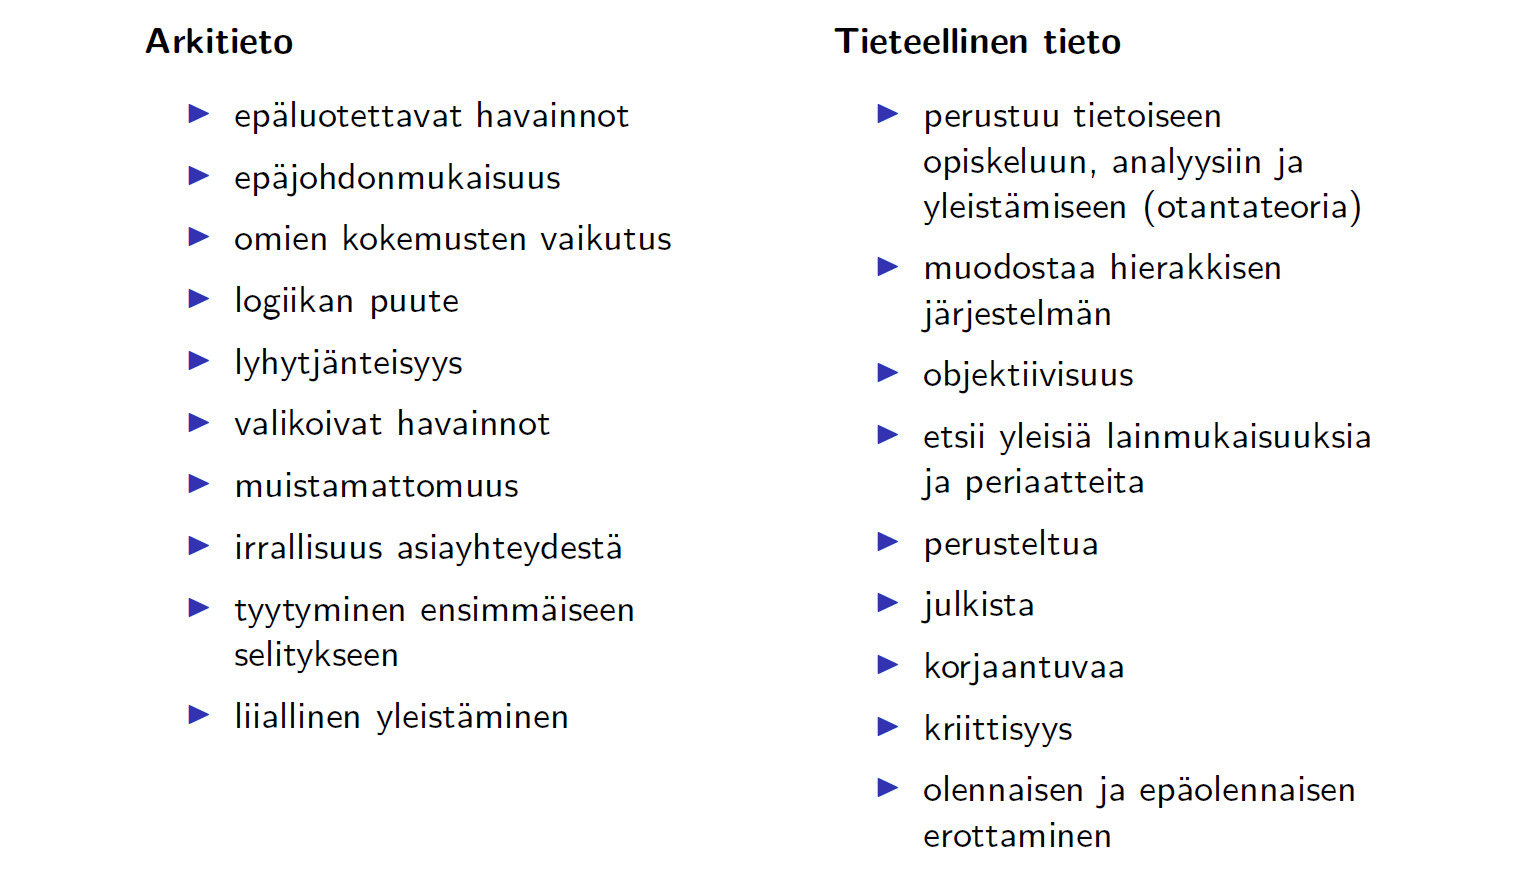
\includegraphics[width=1\linewidth]{images/Arkitieto-tieteellinentieto} 

}

\caption{Arkitieto ja tieteellinen tieto}\label{fig:arki}
\end{figure}

\hypertarget{alaluku22}{%
\section{Tieteellinen menetelmä}\label{alaluku22}}

\begin{itemize}
\tightlist
\item
  Milloin tutkimus sitten on tieteellistä? Tiede on tiedonhankintaa, jossa käytetään erityistä, mahdollisesti tilanteesta (sovelluksesta) riippuvaa, tieteellistä \textbf{menetelmää} eli \textbf{metodia}.
\end{itemize}

\begin{defblock}{}

\textbf{Tieteellinen menetelmä}: Tieteellinen menetelmä on kullakin tieteen alalla vallitseva, ajan myötä kehittynyt ja nykyisten paradigmojen mukainen menettelytapa, jolla uutta tietoa tuotetaan ja vanhaa, mutta epävarmaa tietoa vahvistetaan. Se ei ole selkeä työvaiheiden luettelo tai menetelmähakemisto, vaan yleisesti hyväksytty ja hyväksi todettu tapa pyrkiä totuuteen erilaisten tutkimusongelmien ratkomisessa. Hyvälle tieteelliselle menetelmälle voidaan lukea seuraavia kriteerejä.

\begin{itemize}
\tightlist
\item
  \textbf{Objektiivisuus ja loogisuus}

  \begin{itemize}
  \tightlist
  \item
    Tutkimuskohteen ominaisuudet ovat tutkijan mielipiteistä riippumattomia.
  \item
    Tieteellinen tieto tutkimuskohteesta syntyy tutkijan ja tutkimuskohteen vuorovaikutuksen tuloksena.
  \item
    Tiedon lähteenä on tutkimuskohteesta saatava kokemus.
  \item
    Tutkimuskohteesta voidaan saada totuudellista tietoa, jonka laadusta myös tutkijayhteisö voi olla yhtä mieltä.
  \end{itemize}
\item
  \textbf{Kriittisyys}

  \begin{itemize}
  \tightlist
  \item
    Ilmenee niinä vaatimuksina, joita \textbf{hypoteesin} asettamiselle, testaamiselle ja hyväksymiselle on asetettu.
  \item
    Tieteellisten hypoteesien tulee olla intersubjektiivisesti testattavissa eli niillä täytyy olla yhdessä sopivien lisäoletusten kanssa sellaisia seurauksia, joiden totuus tai virheellisyys voidaan julkisesti tarkistaa.
  \end{itemize}
\item
  \textbf{Autonomisuus}

  \begin{itemize}
  \tightlist
  \item
    Tieteen tulosten arvioiminen on (tiukasti ottaen) tieteellisen yhteisön oma asia, johon tieteen ulkopuolella olevat ryhmät eivät saa vaikuttaa.
  \item
    Ei ole hyväksyttävää vedota siihen, että väitteen totuus olisi toivottavaa tai epätoivottavaa esimerkiksi poliittisista, uskonnollisista tai moraalisista syistä.
  \end{itemize}
\item
  \textbf{Edistyvyys}

  \begin{itemize}
  \tightlist
  \item
    Tieteen edistyminen merkitsee kasvun eli tulosten määrällisen lisääntymisen ohella sitä, että virheellisiä hypoteeseja tai teorioita korvataan uusilla tuloksilla, jotka ovat tosia tai ainakin vähemmän virheellisiä kuin aikaisemmat.
  \end{itemize}
\item
  \textbf{Toistettavuus ja yleistettävyys}

  \begin{itemize}
  \tightlist
  \item
    Tieteen tulokset tulee olla muiden tutkijoiden toistettavissa eli replikoitavissa. Toistettavuudelle (paikoin myös uusittavuudelle, joskin merkitys vaihtelee) on erilaisia määritelmiä.
  \end{itemize}
\end{itemize}

\end{defblock}

\begin{itemize}
\tightlist
\item
  Tarkastellaan lähemmin erästä määritelmää erilaisille toistettavuuden lajeille. Esittelemme tässä Hamermeshin (2007)\footnote{Hamermesh, D. S. (2007). Replication in economics \emph{Canadian Journal of Economics/Revue canadienne d' ́economique} 40 (3), 715--733.} esittämän erilaisten replikointien jaottelun:

  \begin{itemize}
  \tightlist
  \item
    \textbf{Puhdas replikointi}: toinen tutkija, käyttäen täysin samaa tutkimusaineistoa ja samaa tilastollista menetelmää kuin alkuperäisessä tutkimuksessa, saa täsmälleen samat tutkimustulokset.
  \item
    \textbf{Tilastollinen replikointi}: toinen tutkija, käyttäen eri tutkimusaineistoa (otosta), joka on kuitenkin poimittu samasta populaatiosta (ks. Luku \ref{luku5}), mutta samaa menetelmää, saa vastaavanlaisia tuloksia, jotka vahvistavat alkuperäisen tutkimuksen perustulokset.
  \item
    \textbf{Tieteellinen replikointi}: toinen tutkija, käyttäen samoja asioita mittaavaa tutkimusaineistoa, joka on kuitenkin kerätty eri populaatiosta, ja käyttäen samankaltaista, mutta ei identtistä menetelmää, saa vastaavanlaisia tuloksia, jotka vahvistavat alkuperäisen tutkimuksen perustulokset.
  \end{itemize}
\end{itemize}

\hfill\break
\hfill\break

\begin{itemize}
\tightlist
\item
  Teorioiden sisältämiä väitteitä voidaan muotoilla tieteellisiksi malleiksi, joihin voidaan liittää hypoteeseja, joita testataan tieteellisin menetelmin käyttäen ilmiö(i)stä mitattua havaintoaineistoa.

  \begin{itemize}
  \tightlist
  \item
    Tieteelliset mallit ovat yksinkertaistuksia reaalimaailmasta ja ne kuvaavat tutkimuksen aihetta jostain näkökulmasta tarkasteltavana systeeminä.
  \item
    Mallit hyödyntävät matemaattista esitystapaa, sillä se tarjoaa formaalin ja objektiivisen tutkimusaiheen kuvauksen sekä mahdollistaa siihen liittyvän loogisen päättelyn havaitun, empiirisen aineiston pohjalta.
  \item
    Tilastolliset mallit ovat käytännössä tieteellisten mallien formaaleja matemaattisia esityksiä, jotka lisäksi mahdollistavat mallia koskevan tilastollisen päättelyn esimerkiksi hypoteesien ja niiden
    testaamisen avulla. Päättely perustuu tilastotieteen teoriaan, joka mahdollistaa päättelyn epävarman ja satunnaisen aineiston tapauksissa.
  \item
    Hypoteesien testaamisen voidaan ajatella tutkittavaa ilmiötä koskeviksi ennusteiksi, joita verrataan havaittuun aineistoon. Mikäli havaittu aineisto ei sovi testattavaan teoriaan tai siihen liittyviin hypoteeseihin, voidaan teoriaa kehittää paremmaksi. Tämä vuoropuhelu vie tiedettä eteenpäin ja tuottaa lisää tutkittua tietoa ympäröivästä maailmasta.
  \end{itemize}
\item
  Hypoteesien testaaminen on yhtäältä tieteellisten teorioiden kehittämisen ja vahvistamisen ja toisaalta kritiikin keskiössä.

  \begin{itemize}
  \tightlist
  \item
    Metodologinen pluralismi: Kaikkia menetelmiä voi soveltaa hyvin tai huonosti, mutta niitä voi käyttää myös luovasti väärin.
  \end{itemize}
\end{itemize}

\hypertarget{alaluku23}{%
\section{Tilastojen yleisestä roolista yhteiskunnassa}\label{alaluku23}}

\begin{itemize}
\tightlist
\item
  Ihminen ei voi toimia maailmassa järkevästi, ellei hän pysty muodostamaan oikeata kuvaa maailmasta ja sen tilasta. Nykyaikana oikeaa kuvaa varten tarvitaan maailmaa ja sen tilaa merkityksellisesti ja oikein kuvaavia, ajantasaisia \textbf{(tilasto)tietoja}.\\
  ~\\
\item
  Yhteiskunnan kaikilla sektoreilla toiminnan seuranta, päätöksenteko ja ennakointi perustuvat eri sektoreita kuvaaviin \textbf{(tilasto)tietoihin} ja niiden analysoinnissa käytettäviin \textbf{tilastollisiin menetelmiin}.

  \begin{itemize}
  \tightlist
  \item
    Oikein todellisuutta kuvaavat, ajantasaiset (tilasto)tiedot ovat välttämättömiä modernin yhteiskunnan toiminnalle.
  \item
    Esimerkiksi päätöksenteko sekä julkisella että yksityisellä sektorilla (elinkeinoelämässä) perustuu pitkälti yhteiskuntaa ja elinkeinoelämää kuvaaviin (tilasto)tietoihin ja tilastollisten menetelmien tuottamiin tuloksiin sekä niiden perusteella tehtäviin päätöksiin.

    \begin{itemize}
    \tightlist
    \item
      Esimerkkejä ovat tietyt konkreettiset (talous)poliittiset toimenpiteet (talous)tilastojen perusteella. Lisäksi tuotantoprosessien ohjaus ja laadunvalvonta teollisuudessa sekä markkinatutkimus kaupan alalla perustuvat tilastollisiin menetelmiin.
    \end{itemize}
  \item
    (Tilasto)tietojen saatavuutta voidaan pitää jopa toimivan demokratian edellytyksenä.\\
    ~\\
  \end{itemize}
\item
  Koska todellisuutta kuvaaviin (tilasto)tietoihin sisältyy (lähes) aina epävarmuutta ja satunnaisuutta, tilastotiede ja tilastolliset menetelmät luovat perustan tilastojen tuotannolle, jalostukselle ja analysoinnille.

  \begin{itemize}
  \tightlist
  \item
    Niinpä tilastojen tuotannon, jalostuksen ja analysoinnin menetelmien kehittäminen on keskeinen osa tilastotieteen tehtäväkenttää.
  \item
    Samoin tilastotieteen menetelmien ymmärtämisellä on keskeinen rooli tietoyhteiskunnassa toimimisessa ja vaikuttamisessa.\\
    ~\\
  \end{itemize}
\end{itemize}

\begin{eblock}{}

\textbf{Esimerkki (väite)}: Naiset puhuvat enemmän kuin miehet.

\begin{itemize}
\tightlist
\item
  Lähtökohta väitteen (hypoteesin) tutkimiseen:

  \begin{itemize}
  \tightlist
  \item
    Uskomus on väärä kunnes toisin todistetaan.
  \item
    Lähdetään liikkeelle olettamuksesta, että miehet ja naiset puhuvat yhtä paljon.
  \item
    Olettamuksen tueksi tai kumoamiseksi täytyy kerätä todistusaineistoa
  \item
    Jotta tutkimukseen saataisiin täysin varma vastaus, kaikki miesten ja. naisten puheet ihmiskunnan olemassa olon ajalta pitäisi pystyä laskemaan = mahdotonta.
  \end{itemize}
\item
  Mitä siis tehdä?

  \begin{itemize}
  \tightlist
  \item
    Täytyy tyytyä tutkimaan osajoukkoja miehistä ja naisista (otos), mihin tarvitaan \textbf{otantamenetelmiä} (käsitellään tarkemmin myöhemmin luvussa \ref{luku5}).
  \item
    Arvotaan satunnaisesti tutkimushenkilöitä miesten ja naisten joukosta ja mitataan kuinka paljon he puhuvat.
  \item
    Satunnaisuus tärkeää, sillä jos valikoitaisiin tarkoituksella puheliaita tai vähäsanaisia tutkimushenkilöitä, tulokset vääristyisivät.
  \end{itemize}
\item
  Jokaiseen mittaukseen liittyy virhe.

  \begin{itemize}
  \tightlist
  \item
    Täysin satunnainenkaan otos ei edusta täydellisesti koko väestöä. Joukkoon saattaa valikoitua puhtaasti sattumaltakin poikkeuksellisen puheliaita tai harvasanaisia naisia tai miehiä.
  \item
    Millaisia sekoittavia tekijöitä tulee mieleen? Mitkä seikat voisivat vaikuttaa tutkittavaan asiaan?
  \item
    Tosin mitä suurempi otos, sitä pienemmäksi sattuman osuus käy ja joudutaan turvautumaan todennäköisyyksiin: Kun aineisto on kerätty, halutaan tietää kuinka todennäkoistä on, että uskomus pitää paikkaansa.
  \end{itemize}
\item
  Palataan takaisin esimerkkiimme: Yleisen uskomuksen mukaan naiset puhuvat enemmän kuin miehet.

  \begin{itemize}
  \tightlist
  \item
    Tutkimuksen mukaan miehet vaikuttavat kuitenkin puhuvan yhtä paljon kuin naisetkin.
  \item
    Laajemmat tutkimukset osoittavat, että tilanteella on puheen määrään paljon suurempi vaikutus kuin sukupuolella.
  \item
    Kiitos tilastotieteen, väärä uskomus on korvautunut tiedolla!
  \end{itemize}
\end{itemize}

\end{eblock}

\begin{figure}

{\centering 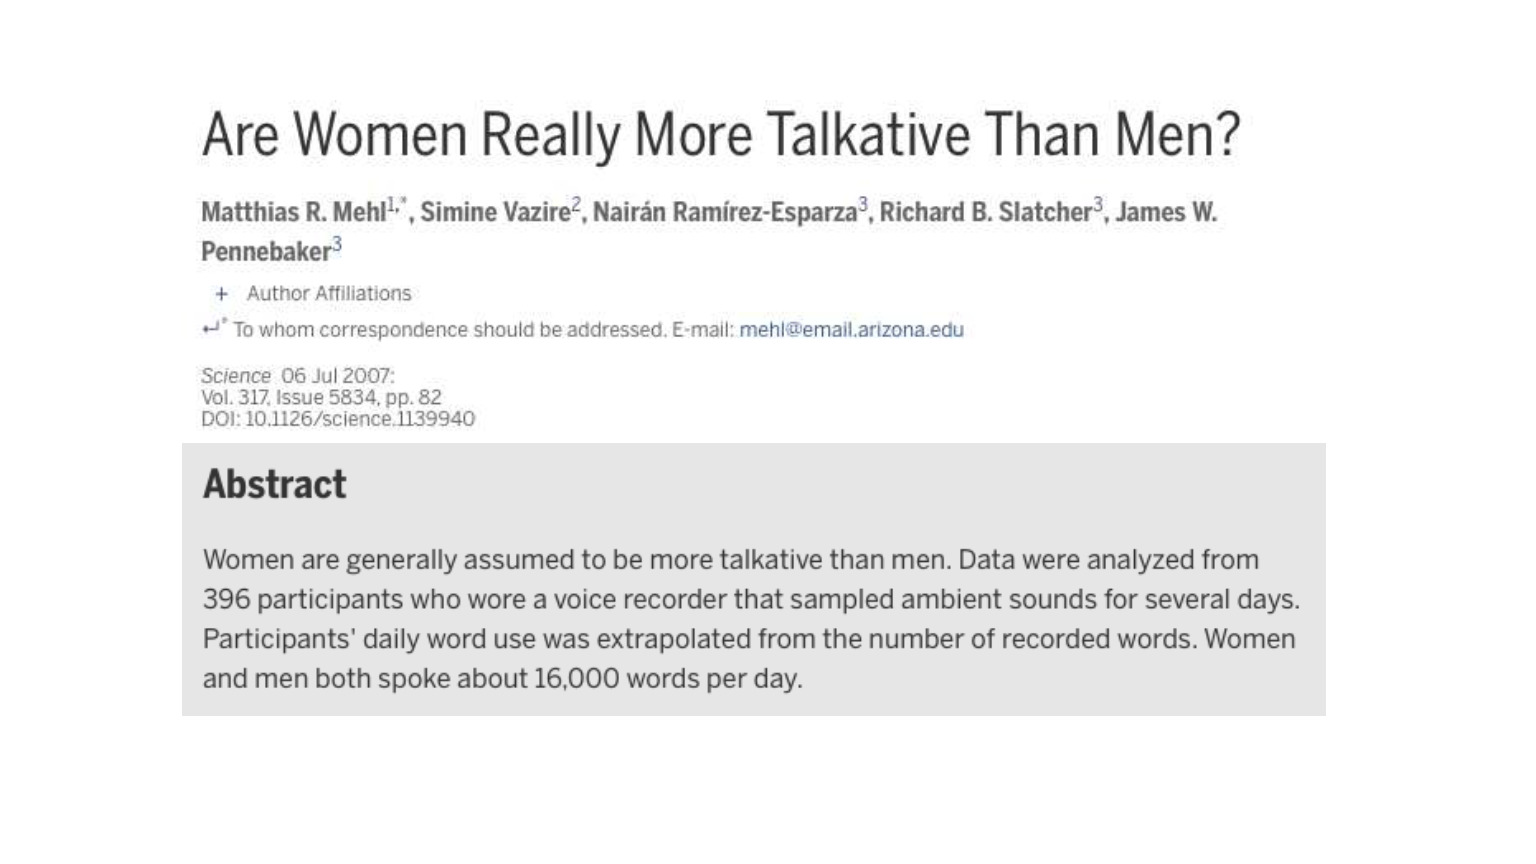
\includegraphics[width=1\linewidth]{images/Are-women-really-more-talkative} 

}

\caption{Are women really more talkative than men?}\label{fig:talkative}
\end{figure}

\hypertarget{alaluku24}{%
\section{Mitä on tutkimus?}\label{alaluku24}}

\begin{itemize}
\tightlist
\item
  Tiede tavoittelee tietoa, mutta mistä?

  \begin{itemize}
  \tightlist
  \item
    Jokaisen tutkimuksen lähtökohtana on (tai ainakin pitäisi useimmiten olla) tiedollisen uteliaisuuden, käytännön tarpeiden tai teorian kehittämispyrkimyksen herättämä ongelma, johon tutkimuksen avulla etsitään vastausta. Tutkimus yrittää käsittää sekä tulkitun ilmiön, että sen tajunnassa synnyttämät spontaanit mielikuvat tai arkipäivän tiedot.
  \item
    Tutkimus siis pyrkii löytämään täysin uutta tietoa, varmentamaan (mahd. aiempien tutkimusten myötä) syntyneitä vallitsevia mutta epävarmoja käsityksiä sekä tarkistamaan vakiintuneen tiedon paikkansapitävyyttä.
  \item
    Valtaosa tieteestä asemoituu erityisesti kahden viimeisen kohdan alaisuuteen vaikka tieteen popularisoinnissa (mm. median toimesta) usein keskitytäänkin uusiin tiedemaailmaa järisyttäviin löydöksiin, jotka tosin voivat usein olla hyvin epävarmoja!

    \begin{itemize}
    \tightlist
    \item
      Lisää tieteen popularisoinnista ja jaksossa \ref{alaluku46}.\\
      ~\\
    \end{itemize}
  \end{itemize}
\item
  Millaisia kysymyksiä \textbf{tutkimuksessa} asetetaan (voidaan asettaa)?

  \begin{itemize}
  \tightlist
  \item
    \textbf{Kuvaus}: Kuinka suuri on yli 65-vuotiaiden osuus Suomen väestöstä?
  \item
    \textbf{Riippuvuuden kuvaus}: Ovatko paljon mainostavat yritykset kannattavampia kuin vähän mainostavat?\\
  \item
    Kuvattujen ilmiöiden \textbf{selittäminen} ja \textbf{ymmärtäminen}. Miksi vanhempien sosioekonominen asema vaikuttaa ekonomien työhönsijoittumiseen? Tämän tutkimuskysymyksen tapauksessa pyrkimys on lähinnä selittää (ymmärtää) ilmiötä.
  \item
    \textbf{Ennustaminen}: Jos kansantulon kasvu pienenee x\%, työttömyyden ennustetaan kasvavan y tuhannella.
  \item
    Kohdetta kuvaavien käsitteiden ja teorioiden rakentaminen, teorioiden ansioiden ja puutteiden arviointi.
  \end{itemize}
\item
  Myöhemmin materiaalissa (luvussa \ref{luku11}) keskustellaan vielä tarkemmin miten tilastotieteessä ilmiön ymmmärtäminen (selittäminen) ja ennustaminen eroavat toisistaan.\\
  ~\\
\item
  \textbf{Tutkimuksen rajat?} Onko niitä?

  \begin{itemize}
  \tightlist
  \item
    Tutkimus antaa aina vajavaisen kuvan tutkimuskohteesta.

    \begin{itemize}
    \tightlist
    \item
      Kehittynytkin tieteellinen teoria tai malli on aina reaalimaailman yksinkertaistus: tutkimus on aina alisteinen käytetylle menetelmälle ja sen oletuksille!
    \end{itemize}
  \item
    Ymmärtämiseen tarvittava havaintomaailman hahmotus (saattaa) tuottaa ideologisesti ja historiallisesti sitoutuneita yksinkertaistavia sekä luonteeltaan usein hyvin teoreettisia abstraktioita.

    \begin{itemize}
    \tightlist
    \item
      Alakohtainen substanssitietous sekä sen vahvuuksien ja puutteiden sekä historiallisen ja ideologisen kontekstin tiedostaminen on ensiarvoisen tärkeää kaikessa tutkimuksessa!
    \end{itemize}
  \item
    Joka tapauksessa täyteen neutraaliuteen ja objektiivisuuteen on mahdotonta päästä. Tästä huolimatta on hyvä ja tärkeää pystyä tunnistamaan tämä haaste.
  \item
    Tutkimusta voi tehdä joistakin arvolähtökohdista, mutta sen tulisi olla näkyvää. Omien arvojen mahdollisimman selvä eksplikointi on yksi keino, jolla voi yrittää vähentää piiloarvojen vaikutusta tutkimukseen.

    \begin{itemize}
    \tightlist
    \item
      Arvot ilmenevät esimerkiksi tutkimuksessa käytetyissä käsitteissä, jotka harvoin ovat arvovapaita. Useimmat käsitteet voidaan korvata toisilla, joilla on paikoin hyvin erilainen arvosisältö joskin arvottava lataus saattaa myös olla paikoin tarkoituksellista! Joka tapauksessa arvopainotteisten valintojen tunnistaminen on vaikeaa.
    \item
      Toisaalta arvoihin sitoutuminen on väistämätöntä, sillä se on sosiaalisen olemassaolon sivutuote. Yhteiskunnan jäseninä meillä on tuskin mahdollisuuksia (täydellisesti) irroittautua arvoistamme kun pyrimme esim. ammatillisiin päämääriin.

      \begin{itemize}
      \tightlist
      \item
        Myös päinvastainen ongelma olemassa: Tutkimusta arvioidaan siihen perustellusti tai perusteettomasti kiinnitettyjen arvonäkökohtien mukaan!
      \end{itemize}
    \end{itemize}
  \end{itemize}
\end{itemize}

\hfill\break
\hfill\break

\begin{itemize}
\tightlist
\item
  Tutkimukseen kuuluu olennaisesti myös oman tutkimustyön kuvaaminen, ts. kertomus siitä, miten esitettyihin tuloksiin on päästy.

  \begin{itemize}
  \tightlist
  \item
    Tämän myötä tieteelliselle ajattelulle on ominaista automaattinen \textbf{itsensä korjaaminen}.
  \item
    Tutkimuskysymys, valitut menetelmät, käytetty aineisto ja tehdyt johtopäätökset perataan auki tutkimusartikkelissa/raportissa, joka sitten lähetetään \textbf{vertaisarvioitavaksi} tietelliseen julkaisuun, jossa muut alan asiantuntijat arvioivat sen ja päättävät hyväksytäänkö se julkaistavaksi.
  \end{itemize}
\item
  \textbf{Vertaisarvioinnissa} yksi tai useampi, tehdystä tutkimuksesta riippumaton, saman alan tutkija lukee ja tarkastaa tehdyn tutkimusartikkelin, arvioi sitä ja suosittaa tietellisen julkaisun arvioinnista vastaavalle päätoimittajalle (editorille) kyseisen artikkelin hyväksymistä tai hylkäämistä.

  \begin{itemize}
  \tightlist
  \item
    Vertaisarviointi ei aina takaa sitä, että julkaistu tutkimus olisi virheetön ja erinomaisesti tehty, vaan myös väärää tietoa pääsee välillä vertaisarviointiprosessin läpi.
  \item
    Tämä ei kuitenkaan poista tieteellisen prosessin luotettavuutta, sillä uusi tieto varmentuu vasta usean samaa tutkimuskysymystä tutkineen ja vastaavat tulokset saaneen tutkimuksen myötä. Toisin sanoen, tieteellisen prosessin voidaan ajatella konvergoituvan totuuteen, vaikka yksittäisiä virhearviointeja sattuisikin.\\
  \end{itemize}
\item
  \textbf{Tutkimuksen kieli}

  \begin{itemize}
  \tightlist
  \item
    Tutkimus edellyttää arkikieltä täsmällisempää kommunikaatiota.
  \item
    Ongelmaan liittyvien käsitteiden huolellinen määritteleminen ja erittely on tarpeellista.

    \begin{itemize}
    \tightlist
    \item
      Käsitteiden ja eri aloilla, osin samoista asioista käytettävien, toisistaan eroavien termien systemaattinen määrittely ja jäsentely selkeyttää tiedeyhteisön välistä kommunikointia.\\
    \item
      Eivät korvaa empiiristä tietoa vaan vaikuttavat tiedon järjestymiseen ja sen perusteella tehtäviin päätelmiin.\\
      ~\\
    \end{itemize}
  \end{itemize}
\end{itemize}

\begin{eblock}{}

\textbf{Esimerkki: Luonnontieteelliset vs.~yhteiskunnalliset sovellutukset}:

\begin{itemize}
\tightlist
\item
  Luonnontieteiden lainalaisuuksia: Monet luonnontieteelliset ilmiöt ovat luonteeltaan varsin pysyviä.

  \begin{itemize}
  \tightlist
  \item
    Voidaan tehdä luotettavasti laajojakin yleistyksiä.
  \item
    Selityksiä voidaan empiirisesti testata.
  \item
    Luotettavia matemaattisia esityksiä voidaan kehittää.
  \end{itemize}
\item
  Yhteiskuntatieteissä (yhteiskuntatieteiden historiallisuuden myötä) erinäisiä lainalaisuuksia ja tyypillisiä piirteitä:

  \begin{itemize}
  \tightlist
  \item
    Usein tutkitaan \textbf{yhteiskunnallisia ilmiöitä}, jotka eivät suurelta osin ole toistettavissa.
  \item
    Vaihtelevat huomattavasti ajan myötä (aiemmin voimassaolleet lainalaisuudet eivät välttämättä ole enää voimassa ja päinvastoin), mikä vaikeuttaa tilastollista analyysiä.
  \item
    Yhteiskunnallisten ilmiöiden mittaaminen?

    \begin{itemize}
    \tightlist
    \item
      Yhteiskunnan rakenne ja toiminta on ehdollinen siinä käytettävän merkitysjärjestelmän suhteen. Kysymys \textbf{mittaamisesta} on asetettava suhteessa tähän käsitejärjestelmään. Joudutaan tekemään erilaisia kompromisseja eksaktisuus- ja systemaattisuusvaatimusten sekä arkikielen monimerkityksellisyyden välillä.
    \end{itemize}
  \end{itemize}
\end{itemize}

\end{eblock}

\hypertarget{alaluku25}{%
\section{Tutkimuksen vaiheet ja tulosten julkaiseminen}\label{alaluku25}}

Tieteellinen tutkimus ja asiantuntijatyö tuottavat valtavan määrän perusteltua, luotettavaa tutkimustietoa. Ks. tarkemmin tieteellisestä julkaisemisesta linkin tapauksessa erityisesti yhteiskuntatieteiden alalla, mutta perusperiaatteet pätevät myös muiden tieteenalojen tapauksessa

\url{https://blogs.uef.fi/tiedonhaku-yhteiskuntatiede/tieteelliset-julkaisut/}~\\

Vastuullisen tieteen

\url{https://vastuullinentiede.fi/fi/julkaiseminen}

artikkelit tarjoavat tietoa siitä, kuinka tutkittua tietoa tuotetaan, julkaistaan ja arvioidaan luotettavasti ja yhteisesti hyväksytyllä tavalla. Jotta tiede vaikuttaa koko yhteiskunnan hyväksi, toiminnan on oltava vastuullista tutkimuksen jokaisessa vaiheessa.

Helsingin Yliopisto tarjoaa lisäksi \href{https://tiedelukutaito.mooc.fi/}{Tiedelukutaidon perusteet -kurssia} MOOC-toteutuksena (Massive Open Onlince Course). Keskustelethan ennen kurssin käymistä oman alasi koulutussuunnittelijan (tai vastaavan vastuuhenkilön) kanssa siitä, soveltuuko kyseinen kurssi sisällytettäväksi johonkin omaan opintokokonaisuuteesi.

\hfill\break
\hfill\break

\begin{itemize}
\tightlist
\item
  Julkisuus ja avoimuus tekevät tutkimuksesta tiedettä.
\item
  Tiedeviestintä on tiedeyhteisöjen sisäistä ja ulkoista tiedonvälitystä ja vuorovaikutusta. Tutkimuksesta viestiminen ei ole vain tutkimustuloksista viestimistä. Vastuullinen tiedeviestintä lisää luottamusta tieteelliseen tietoon.
\item
  Tieteellinen julkaiseminen on tutkijoille tärkeä meritoitumisen tapa, ja siksi on tärkeää, että tekijyys määritellään niin, että se palkitsee tutkijat oikeudenmukaisesti.
\end{itemize}

\hypertarget{luku3}{%
\chapter{Tilastotiede tieteenalana}\label{luku3}}

Tässä luvussa hahmottelemme tilastotieteen piirteitä tieteenalana. Käymme läpi tilastotieteelle ominaisia piirteitä, jotka erottavat sen niin lähitieteistä, kuten matematiikasta ja tietojenkäsittelytieteestä, kuin myös sovellusaloista. Usein näkee tilastotieteen typistettävän vain työkaluksi eri sovellusalojen empiiriseen tutkimukseen siitäkin huolimatta että tilastotieteellä on oma rikas teoriapohjansa sekä kiistaton asema omana tieteenalanaan.

Tieteenalan määritteleminen lyhyesti on aina hieman hankalaa. Tästä huolimatta seuraavassa yritämme osaltaan vastata seuraaviin kysymyksiin:

\begin{itemize}
\tightlist
\item
  Mitä tilastotiede on ja mitä se ei ole? Miksi tilastotiede ei ole vain sovellettua matematiikkaa tai matematiikalla höystettyä tietojenkäsittelyä?
\item
  Mihin tilastotiedettä käytetään? Onko tilastotieteellä käyttöä ns. ``akatemian'' eli tutkimusyhteisön ulkopuolella?
\item
  Minkälaista on tyypillinen tilastotiedettä kohtaan esitetty kritiikki?
\end{itemize}

\hypertarget{alaluku31}{%
\section{Lisää tilastotieteen perustermejä}\label{alaluku31}}

Seuraavia tilastotieteen esittelyä ja karakterisointeja ajatellen määritellään seuraavassa lisää tilastotieteellisen tutkimuksen peruskäsitteitä. Näihin käsitteisiin paneudutaan osaltaan tarkemmin mm. luvussa \ref{luku5}.

\begin{itemize}
\tightlist
\item
  Tilastotieteellinen tutkimus tarkastelee reaalimaailman ilmiöitä. Täten tutkimuskohteena on tavallisessa elämässä tavattavia asioita, ihmisiä tai tapahtumia. Tutkimuskohteita kutsutaan tilastoyksiköiksi ja niiden joukkoa kutsutaan populaatioksi (perusjoukoksi).

  \begin{itemize}
  \tightlist
  \item
    Esimerkiksi jos tutkitaan kuntavaaleissa äänestävien tuloja niin jokainen äänestysikäinen muodostaa oman tilastoyksikkönsä (ks. alla) ja täten populaationa (perusjoukkona) toimii kaikki äänestysikäiset kansalaiset. Jos taas tutkitaan äänestysaktiivisuutta eri kunnissa, muodostaa jokainen kunta oman tilastoyksikkönsä ja kaikki Suomen kunnat muodostavat populaation.
  \end{itemize}
\end{itemize}

\begin{defblock}{}
\textbf{Populaatio}

Konkreettinen tai hypoteettinen tutkimuskohteiden joukko, joka koostuu kaikista tilastoyksiköistä

\end{defblock}

\begin{itemize}
\tightlist
\item
  Populaation muodostavilta tilastoyksiköiltä tarkastellaan niiden ominaisuuksia, eli \textbf{tilastollisia muuttujia}.

  \begin{itemize}
  \tightlist
  \item
    Edellisissä esimerkeissä nämä olisivat esim. äänestäjien tulot ja kuntien äänestysprosentti.
  \item
    Mielenkiinnon kohteena olevia tilastollisia muuttujia kutsutaan \textbf{tutkimusmuuttujiksi} (tulot ja kuntien äänestysprosentti) ja niiden lisäksi voidaan kerätä ylimääräistä tietoa eli \textbf{taustamuuttujia} (näitä voisi olla esimerkiksi asuinpaikka ja kunnan väkiluku).
  \item
    Tilastoyksiköiden tilastollisilla muuttujilla on tietty mahdollisten arvojen joukko, ja näillä arvoilla on jokin \textbf{jakauma} populaatiossa.

    \begin{itemize}
    \tightlist
    \item
      Esimerkiksi tulot voivat määritelmästä riippuen saada minkä tahansa positiivisen arvon mutta äänestysprosentti on luonnollisesti rajattu nollan ja sadan prosentin väliin.
    \end{itemize}
  \end{itemize}
\end{itemize}

\begin{defblock}{}
\textbf{Tilastoyksikkö ja tilastollinen muuttuja}

Populaation muodostavilta tilastoyksiköiltä (populaation alkioilta) tarkastellaan tilastollisia muuttujia, joita voidaan mitata tai havaita.

\end{defblock}

\begin{itemize}
\tightlist
\item
  Kun tarkasteltavien tilastoyksikön tilastollisten muuttujien (numeeriset) arvot havaitaan, kutsutaan näiden arvojen joukkoa \textbf{havainnoksi}
\end{itemize}

\begin{defblock}{}
\textbf{Havainto}

Havainto muodostuu tilastoyksikön tarkasteltavien tilastollisten muuttujien havaitusta arvoista.

\end{defblock}

\begin{itemize}
\tightlist
\item
  Kerättyjen havaintojen joukko muodostaa \textbf{havaintoaineiston}, eli \textbf{datan}.
\end{itemize}

\begin{defblock}{}
\textbf{Havaintoaineisto/data}

Havaintoaineisto, data, on tilastoyksiköiden tilastollisista muuttujista kerätty havaintojen joukko.

\end{defblock}

\textbf{Tiivistettynä}:

\begin{itemize}
\tightlist
\item
  Populaatio koostuu tutkimuksen kohteena olevista tilastoyksiköistä.
\item
  Havaitaan tilastoyksiköistä tutkimuksen kannalta mielenkiintoisia tilastollisten muuttujien numeerisia arvoja.
\item
  Nämä havainnot muodostavat havaintoaineiston, eli datan, jota voidaan käyttää tutkimuksessa ja tutkia \textbf{populaation ominaisuuksia}.
\end{itemize}

\hypertarget{alaluku32}{%
\section{Mitä tilastotiede on ja mitä se ei ole?}\label{alaluku32}}

\begin{itemize}
\tightlist
\item
  Aloitetaan tarkastelemalla erinäisiä \textbf{tilastotieteen ``karakterisointeja''} eri tahojen ja tutkijoiden toimesta:

  \begin{itemize}
  \tightlist
  \item
    \textbf{\emph{Tilastotiede on tietotuotannon teknologiaa}}, \emph{jonka avulla voidaan suorittaa kvantitatiivisten tietojen joukkotuotantoa ja havaintoihin perustuvia tieteellisiä ja käytännöllisiä päätöksiä. Tilastotiede on siis yksikköjen muodostamaan joukkoon liittyvän numeerisen tietoaineiston keräämistä, analysointia ja tulkintaa koskeva tiede} \footnote{\href{https://fi.wikipedia.org/wiki/Leo_T\%C3\%B6rnqvist}{Leo Törnqvistin}, Suomen ensimmäisen tilastotieteen professorin, esittämä luonnehdinta (Vartia, 1989).}.
  \item
    \textbf{\emph{Tilastotiede on yleinen menetelmätiede}}, \emph{jota sovelletaan, jos reaalimaailman ilmiöstä halutaan tehdä johtopäätöksiä ilmiötä kuvaavien kvantitatiivisten tai numeeristen tietojen perusteella sellaisissa tilanteissa, joissa tietoihin liittyy epävarmuutta tai satunnaisuutta} \footnote{Mellin, (2005).}.
  \item
    \textbf{\emph{Tilastotiede on yleinen menetelmätiede}}, \emph{jota sovelletaan, jos reaalimaailman ilmiöstä halutaan tehdä johtopäätöksiä ilmiötä kuvaavien kvantitatiivisten tai numeeristen tietojen perusteella sellaisissa tilanteissa, joissa tietoihin liittyy epävarmuutta tai satunnaisuutta.}
  \item
    \emph{Vale, emävale, tilasto} \footnote{\href{https://fi.wikipedia.org/wiki/Mark_Twain}{Mark Twain} popularisoi tämän lausahduksen teoksessaan \emph{Chapters from My Autobiography} jo vuonna 1907. Huomionarvoista toki on, että valtaosa ``modernin'' tilastotieteen, jolle nykytilastotiede pohjautuu, teoriakehityksestä on tapahtunut vasta Twainin teoksen julkaisun jälkeen. Esimerkiksi Ronald Fisher, jota pidetään modernin tilastotieteen isänä, julkaisi merkityksellisimmät työnsä vasta 1920- ja 30-lukujen aikana, joten tällä lentävällä lausahduksella ei ole mitään tekemistä nykyisten tilastollisten menetelmien kanssa.}.
  \item
    \emph{Statistics concerns what can be learned from data} \footnote{(A.C. Davison)}.
  \item
    \emph{``Maalaisjärjen tehostamista''} \footnote{(Sund, 2003)}.
  \end{itemize}
\item
  Tilastotiede siis \textbf{kehittää} ja \textbf{soveltaa menetelmiä} ja (tilastollisia) \textbf{malleja}, joiden avulla reaalimaailman ilmiöistä voidaan tehdä johtopäätöksiä ilmiöitä kuvaavien numeeristen tai kvantitatiivisten tietojen perusteella tilanteissa, joissa tietoihin liittyy \textbf{epävarmuutta ja satunnaisuutta}.

  \begin{itemize}
  \tightlist
  \item
    Tilastollisten menetelmien avulla pyritään löytämään reaalimaailman satunnaisia ilmiöitä kuvaavista numeerisista (eli kvantitatiivisista) tiedoista \textbf{systemaattisia piirteitä} joita jalostetaan sellaiseen muotoon, että ilmiöistä voidaan tehdä päätelmiä.

    \begin{itemize}
    \tightlist
    \item
      Vrt. signaalin ja kohinan erottaminen (ks. Silver, 2014)\footnote{Silver, N. (2014). Signaali ja kohina: Miksi monet ennusteet epäonnistuvat mutta jotkin eivät? Terra Cognita. (Suomentanut Kimmo Pietiläinen)}.
    \end{itemize}
  \item
    Tilastolliset mallit perustuvat todennäköisyyslaskentaan ja niillä mallinnetaan reaalielämän ilmiöiden alla piileviä prosesseja tai mekanismeja. Näiden prosessien tuottamia tietoja (aineistoja) tiivistetään usein graafisiksi esityksiksi ja tunnusluvuiksi sekä tilastollisten mallien parametreiksi, joiden pohjalta johtopäätöksiä tehdään.
  \item
    Tässä onnistuakseen tilastollisten menetelmien tuleekin pyrkiä erottelemaan \textbf{sattuma} ja \textbf{systemaattisuus} tarkasteltavissa ilmiöissä tai, tarkemmin, niitä kuvaavissa aineistoissa, jotta johtopäätökset olisivat luotettavia.
  \end{itemize}
\end{itemize}

\hfill\break

\textbf{Voidaan sanoa, että saadakseen tarkemmin selville mitä tilastotiede on, pitää opiskella tilastotiedettä ja sen käyttöä!}

\hfill\break

\textbf{Mitä tilastotiede ei ole}

\begin{itemize}
\tightlist
\item
  \textbf{Tilastotiede ei ole vain tilastojen tuotantoa}

  \begin{itemize}
  \tightlist
  \item
    Vaikka sana \textbf{tilasto} tuo useimmille ensimmäisenä mieleen yhteiskuntaa ja sen toimintaa kuvaavat \textbf{numeeristen tietojen järjestelmälliset kokoelmat}, tilastotiede ei suinkaan ole ainoastaan tilastojen ja niiden tekemisen oppia.

    \begin{itemize}
    \tightlist
    \item
      Tämä siitäkin huolimatta, että niiden menetelmien konstruointi, joilla näitä tilastoja tuotetaan, jalostetaan ja analysoidaan on keskeinen osa tilastotiedettä. Tilastot ovat siis usein tilastotieteen soveltajan tutkimuskohteena ja tilastojen laadinnassa käytetään apuna tilastotieteen menetelmiä.
    \item
      Suomessa \href{https://www.stat.fi/}{Tilastokeskus} toimii virallisena tilastoviranomaisena ja tilastotuottajana. Tätä \textbf{tilastotuotannon} kokonaisuutta nimitetään ajoittain \textbf{tilastotoimeksi}. \textbf{Tilastotieteen käyttöalue on paljon tätä laajempi}.
    \item
      Terminologiaa:

      \begin{itemize}
      \tightlist
      \item
        Tilastoala = Tilastotiede + Tilastotoimi\\
      \item
        Tilastotiede = Teoreettinen tilastotiede + Soveltava tilastotiede\\
      \item
        Tilastotoimi = Tilastojen tuotanto + Tilastojen hyödyntäminen
      \end{itemize}
    \end{itemize}
  \end{itemize}
\item
  Tilastotieteen kannalta mikä tahansa reaalimaailman ilmiötä kuvaava \textbf{numeeristen tai kvantitatiivisten tietojen järjestelmällinen kokoelma} voi muodostaa \textbf{tilastollisen aineiston} ja siten tilastollisen tutkimuksen mahdollisen kohteen.

  \begin{itemize}
  \tightlist
  \item
    Esimerkiksi kaikki \textbf{empiirisen} tai \textbf{kvantitatiivisen} tutkimuksen tutkimus- tai havaintoaineistot ovat tilastotieteen kannalta tilastollisia aineistoja.
  \end{itemize}
\end{itemize}

\hfill\break

\begin{itemize}
\tightlist
\item
  Tilastotiede sijoittuu tieteiden kentässä matematiikan, filosofian ja tietojenkäsittelytieteen rinnalle. Tästä huolimatta se ei kuitenkaan ole yksiselitteisesti minkään näiden osa-alue.

  \begin{itemize}
  \tightlist
  \item
    \textbf{Tilastotiede ei ole matematiikan osa-alue}, sillä tilastotiede lähestyy tieteellistä ongelmanratkaisua eri tavoin:

    \begin{itemize}
    \tightlist
    \item
      Matematiikka on tietyllä tavalla aina eksaktia ja sen tulokset perustuvat formaaliin deduktioon ja loogisiin todistuksiin, johtaen usein ``eksaktiin'' ratkaisuun tai matemaattisesti formaaliin ratkaisun loogiseen esitystapaan. - Tilastotiede sen sijaan on aina konteksti- ja aineistopohjaista ja perustuu induktiiviseen päättelyyn. Saadut tulokset ovat aina epävarmoja - koska ne kuvailevat epävarmaa tietoa generoivia prosesseja!

      \begin{itemize}
      \tightlist
      \item
        Tilastotiede on siis hyvä nähdä omana tieteenalanaan matemaattisesta esitystavastaan huolimatta. Eihän esimerkiksi myöskään fysiikkaa (sentään) pidetä matematiikan osa-alueena!
      \end{itemize}
    \end{itemize}
  \item
    \textbf{Tilastotiede ei ole myöskään tietojenkäsittelytieteen osa-alue}, vaikkakin useiden laskennallisten menetelmien ja tehokkaan tietojenkäsittelyn rooli tilastollisissa analyyseissä on jatkuvasti kasvanut.

    \begin{itemize}
    \tightlist
    \item
      Tietojenkäsittelytieteen teoria ei rakennu tilastotieteen tavoin ajatukselle epävarmoista ja satunnaisista reaalimaailman ilmiöistä.
    \end{itemize}
  \end{itemize}
\item
  Vaikka nämä ja jotkin muut alat jakavat tilastotieteen kanssa useita piirteitä ja ominaisuuksia, on tilastotiede kuitenkin siis perustellusti oma tieteenalansa. Tämä erottelun vaikeus jo itsessään todistaa kuinka keskeinen rooli tilastotieteellä on eri aloilla!

  \begin{itemize}
  \tightlist
  \item
    Tilastotiede ei siis kuulu yksiselitteisesti sen lähitieteiden alle, vaan muodostaa oman tieteenalan omine teorioineen ja tieteellisine premisseineen. Käsittelemme myöhemmin tilastotieteen roolia matematiikan ja/tai datatieteiden (``data science'') kokonaisuudessa ja keskustelemme tarkemmin näiden erojen luonteesta.
  \end{itemize}
\end{itemize}

\hfill\break
\hfill\break

\textbf{Mitä tilastotiede (ainakin) on}

\begin{itemize}
\tightlist
\item
  \textbf{Tilastotiede yleisenä menetelmätieteenä}

  \begin{itemize}
  \tightlist
  \item
    Tieteellistä tietoa ympäröivästä maailmasta hankitaan tieteellisillä \textbf{menetelmillä/metodeilla} (Ks. tieteellisen menetelmän kriteerit luku \ref{luku2})), joiden avulla tutkitaan jotain ilmiötä tai sen generoimaa kvantitatiivista mutta epävarmaa tietoa sisältävää aineistoa.
  \item
    Tilastotieteessä kehitetyt ja kehitettävät menetelmät antavat tutkijoille yhtenevät ja tiedeyhteisön hyväksymät raamit, jotka mahdollistavat (tilastollisen) päättelyn ja päätöksenteon epävarman tiedon vallitessa. Näin voidaan uskottavasti ja luotettavasti tiivistää tietoa, jota erilaiset aineistot sisältävät, perustaa johtopäätöksiä näille tiivistyksille ja saavuttaa uusia tieteellisiä löytöjä.

    \begin{itemize}
    \tightlist
    \item
      Tilastotieteen menetelmien käyttö ja soveltaminen onkin siis aina alakohtaista. Tästä huolimatta tilastollisia menetelmiä sovelletaan aina johonkin \textbf{aineistoon}!
    \end{itemize}
  \item
    Tilastotieteen nähdäänkin usein kuuluvan ns. \textbf{menetelmätieteisiin}, joissa mm.:

    \begin{itemize}
    \tightlist
    \item
      Kehitetään työkaluja muiden tieteiden tutkimusongelmien ratkaisuksi
    \item
      On myös oma sovelluksista vapaa teorianmuodostuksensa
    \end{itemize}
  \item
    Menetelmäkehityksen näkökulma tilastotieteeseen: \emph{tilastotiede kehittää matemaattisia} \textbf{\emph{malleja}} \emph{satunnaisilmiöitä kuvaavia kvantitatiivisia tietoja generoiville prosesseille.} Koska tietoihin liittyy \textbf{epävarmuutta} tai \textbf{satunnaisuutta}, \textbf{tilastolliset mallit} perustuvat \textbf{todennäköisyyslaskentaan}.

    \begin{itemize}
    \tightlist
    \item
      Juuri sattuman ja epävarmuuden huomioiminen tutkimusasetelmissa erottaa tilastotieteen muista menetelmätieteistä!
    \end{itemize}
  \end{itemize}
\item
  Tilastollisia menetelmiä voidaan soveltaa tietojen keruun, jalostuksen ja analysoinnin jokaisessa vaiheessa. Päämääränä on jalostaa tiedot muotoon, joka mahdollistaa tutkittavaa reaalimaailman ilmiötä koskevien johtopäätösten tekemisen käytettyjen menetelmien pohjalta, eli ns. \textbf{tilastollisen päättelyn}.

  \begin{itemize}
  \tightlist
  \item
    Tutkimuksessa on pystyttävä valitsemaan ja käyttämään menetelmiä, jotka antavat aineistosta vastauksia haluttuihin kysymyksiin. Tämä vaatii yhtä lailla sovellusalakohtaista osaamista (ns. substanssiosaamista) kuin myös kattavaa menetelmäosaamista.
  \end{itemize}
\end{itemize}

\hfill\break
\hfill\break

\begin{itemize}
\tightlist
\item
  Tilastotieteessä lähtökohtana ja ratkaisevassa asemassa on siis aina jonkin satunnaisilmiön generoima \textbf{aineisto}, josta haluamme oppia tai tietää lisää, kenties voidaksemme tehdä suuria yhteiskunnallisia päätöksiä sen pohjalta!

  \begin{itemize}
  \tightlist
  \item
    Tämä aineistokeskeisyys yhtäältä erottaa tilastotieteen rajatieteistään ja toisaalta tuo sen lähemmäksi niitä ja sovellusalojaan.
  \item
    Aineistoa analysoidaan, kuvaillaan ja mallinnetaan tilastollisin menetelmin, joiden kehittäminen on keskeinen osa tilastotiedettä.
  \item
    Pelkkä menetelmien kehittäminen kuuluu pitkälti matemaattisen/teoreettisen tilastotieteen osa-alueelle.
  \item
    Pelkkä ainestoon keskittyminen ja (mekaaninen) analysointi voi sen sijaan olla joissain tilanteissa pitkälti tietojenkäsittelyä.
  \item
    \textbf{Tilastollinen ``mallintaminen''} löytyykin näiden välistä ja se sisältää eri alojen sovelluksista kumpuavan tarpeen uusien menetelmien kehittämiseen.

    \begin{itemize}
    \tightlist
    \item
      Tämä vuoropuhelu muodostaa tilastotieteelle luonnollisen ``takaisinkytkennän'' teoreettisen ja soveltavan puolen välillä: uudet teoreettiset menetelmät vastaavat soveltavan tilastotieteen ongelmiin mutta herättävät aina uusia kysymyksiä, jotka palautuvat taas teoreettisen tilastotieteilijän pöydälle!
    \end{itemize}
  \item
    Luonnollisesti valtaosa tilastotieteilijöistä ja lähitieteiden harrastajista asettuvat näiden äärimmäisten luonnehdintojen välimaastoon eikä tarkkaa luokittelua ole sinänsä tarpeen tehdä ja korostaa.
  \item
    Joka tapauksessa tilastotieteen kehityksen keskiössä ovat aina sovellusalakohtaiset ongelmat, joista useat palautuvat yleisemmälle tasolle teoreettisen tilastotieteen kehityspolkuihin.
  \end{itemize}
\end{itemize}

\hypertarget{alaluku33}{%
\section{Tilastotieteen suhde lähitieteisiin}\label{alaluku33}}

\begin{itemize}
\tightlist
\item
  Kuvio \ref{fig:datasc} tarjoaa karkean yleistyksen tietojenkäsittelytieteen (Computer Science) ja sovellusalan (Application domain) sekä tilastotieteen (Statistics) ja matematiikan (Mathematics) välisistä yhteyksistä. On selvää että tilastotieteellä on paljon päällekäisyyksiä lähitieteidensä kanssa ja joskus näkeekin (huolimatta edellä tehdyistä huomioista) että tilastotiede niputetaan yhteen matematiikan tai tietojenkäsittelytieteen kanssa.
\end{itemize}

\begin{figure}

{\centering 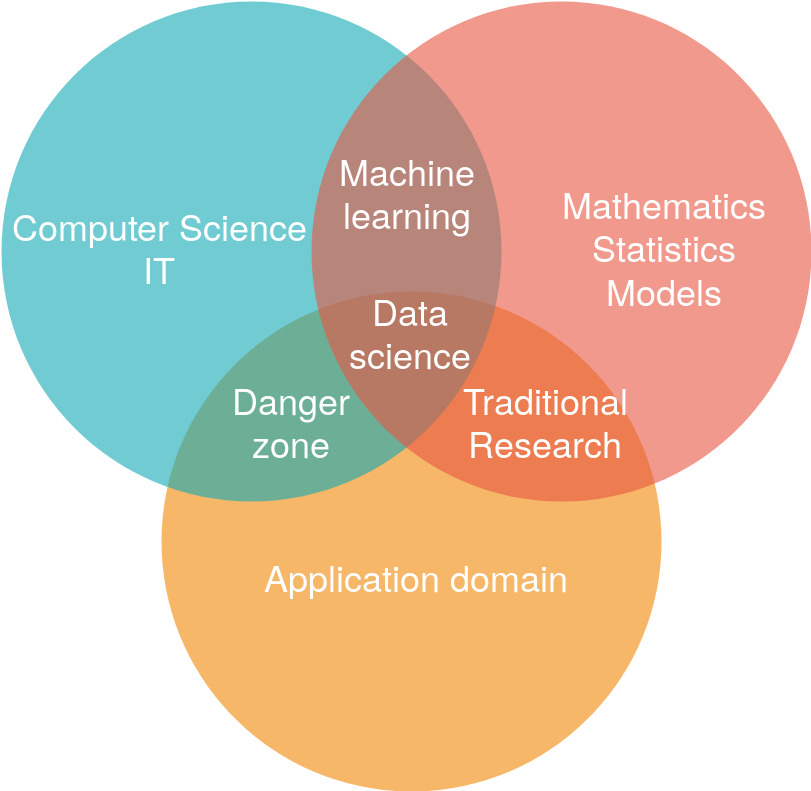
\includegraphics[width=1\linewidth]{images/data_science} 

}

\caption{Tilastotieteen ja rajatieteiden yhteyksiä kuvaava Venn-diagrammi}\label{fig:datasc}
\end{figure}

\begin{itemize}
\tightlist
\item
  Yritetään siis vielä hahmotella tilastotieteen suhdetta sitä lähimpänä olevaan (soveltavaan) matematiikkaan.

  \begin{itemize}
  \tightlist
  \item
    Tilastotieteessä olennaisen otantateorian (Luku \ref{luku5}) voisi ajatella olevan matemaattisesti määritelty teoria, jossa myös on aineiston käsite, mutta se ei tee siitä vielä varsinaisesti tilastotiedettä.
  \item
    Matematiikassa kuvataan ongelma ja esitetään se teorian muodossa, eli malli on \emph{``parametreista havaintoihin''}.
  \item
    Tilastotieteessä ongelma on käänteinen, edetään \emph{``havainnoista parametreihin''}, mutta ongelman matemaattinen kuvaus vaaditaan ensin.
  \item
    Tilastotiede esittää menetelmiä ja käsitteitä tämän käänteisen ongelman ratkaisemiseen.

    \begin{itemize}
    \tightlist
    \item
      Karkeasti erotellen tilastotieteessä käsiteltävät ongelmat lähtevät aina havainnoista eli aineistosta ja matematiikassa suunta on teoriasta aineistoon.
    \item
      Voidaankin siis sanoa, että tilastotieteen erottaa puhtaasta matematiikasta se, että siinä tutkitaan metodeja, jotka mahdollistavat päättelyn/tiedon hankinnan puutteellisesta tai epävarmasta tiedosta.
    \end{itemize}
  \end{itemize}
\item
  Ilmiöiden kuvaamiseen ja käyttäytymisen ennakoimiseen käytetään usein \textbf{mallia}. Mallit (matemaattiset/tilastolliset mallit) voidaan jakaa \textbf{deterministisiin} ja \textbf{stokastisiin} malleihin.

  \begin{itemize}
  \tightlist
  \item
    Deterministisen mallin tapauksessa, tiettyjen alkuehtojen (alkuarvojen) vallitessa voidaan määrittää tarkaltevan ilmiön lopputulos. Esimerkkejä ovat esim. monet fysiikan lait.
  \item
    Stokastiset mallit perustuvat todennäköisyyslaskentaan. Stokastisia malleja käytetään kun alkuehtojen perusteella ei voida varmasti määrittää tarkasteltavan ilmiön lopputulosta. Tällöin eri vaihtoehtoihin liittyvät tietyt esiintymistodennäköisyydet. Esimerkkejä ovat esim. rahanheitto tai sään ennustaminen.
  \item
    Kun jotain ilmiötä kuvataan stokastisen mallin avulla, voidaan käyttää (joudutaan käyttämään) tilastollisia menetelmiä. Vaikka käytännössä laskenta hoidetaan tietokoneohjelmien avulla, meidän tilastotieteen tutkijoina ja käyttäjinä on huolehdittava tutkimusprosessin onnistuneesta toteutuksesta muilta osin.
  \end{itemize}
\end{itemize}

\hfill\break
\hfill\break

\begin{itemize}
\tightlist
\item
  Tilastotiede ei myöskään ole puhtaasti tietojenkäsittelyä, vaikka tilastotiede onkin luonteeltaan aineistopohjaista ja aineistojen sisältämää tietoa on käsitelty osin samoin kuin tietojenkäsittelyssä siitä asti kun se on ollut mahdollista (tietokoneen keksimisen myötä).

  \begin{itemize}
  \tightlist
  \item
    Tilastotieteen ja tietojenkäsittelytieteen ero on lähitieteistä selvin: tilastotieteellä on ``mekaanisesta'' tai teoreettisesta tietojenkäsittelystä selkeästi erillinen ja oma teoriapohjansa.

    \begin{itemize}
    \tightlist
    \item
      Siinä missä tilastotieteen teoria perustuu aineiston stokastiselle mallintamiselle, tietojenkäsittely on enemmänkin algoritmista ajattelua, missä aineistolla on ratkaisevalla tavalla erilainen rooli.
    \end{itemize}
  \item
    Lisäksi suomen kielessä tietojenkäsittely ymmärretään laajemmassa mielessä ohjelmoitavissa olevaksi automatisoimiseksi, jota tilastotiede ei perusolemukseltaan suinkaan ole.
  \end{itemize}
\end{itemize}

\hfill\break
\hfill\break

\begin{itemize}
\tightlist
\item
  Tarkastellaan seuraavaksi tilastotieteen suhdetta viime vuosien aikana paljon suosiota keränneeseen datatieteeseen (data science) johon voidaan katsoa lukeutuvan mm.

  \begin{itemize}
  \tightlist
  \item
    Tilastotiede ja matematiikka

    \begin{itemize}
    \tightlist
    \item
      Erityisesti tilastollinen data-analytiikka ja satunnaisen aineiston mallintaminen sekä soveltuvat soveltavan matematiikan osa-alueet.
    \end{itemize}
  \item
    Tietojenkäsittely

    \begin{itemize}
    \tightlist
    \item
      Tietoteknologian kehityksen myötä taitavien tietojenkäsitteljöiden kysyntä on kasvanut merkittävästi. Lähes jokaisella alalla kerätään entistä enemmän dataa lähes kaikesta, jonkun pitäisi osata myös käsitellä sitä!
    \item
      Datatieteen voidaankin osaltaan katsoa syntyneen tästä elinkeinoelämän tarpeesta asiantuntijoille, jotka osaavat käsitellä suuria tietoaineistoja (dataa) sekä mallintaa niitä hyödyllisellä tavalla.
    \end{itemize}
  \item
    Sovellusala

    \begin{itemize}
    \tightlist
    \item
      Datatiede on luonteeltaan pääosin soveltavaa ja sen alaan lukeutuvia menetelmiä sovelletaan aina johonkin tosielämän ongelmaan. Tästä syystä nk. substanssiosaaminen sovellusalalta on datatieteilijälle erityisen tärkeää ja nykypäivänä datatieteilijän rooli onkin pirstaloitunut yhä enemmän eri sovellusalojen datatieteisiin.
    \item
      Tästä huolimatta datatieteilijöiden käyttämät mallinnusmenetelmät ovat usein varsin samanlaisia, sillä ne pohjautuvat edelleen tilastotieteen ja matematiikan teoriapohjaan. Ilman jälkimmäisten riittävää osaamista, liikutaan datatieteen osalta vaarallisilla vesillä! (Ks. alta).\\
    \end{itemize}
  \end{itemize}
\item
  Datatieteellä ei usein nähdä olevan omaa historiallisen tieteellisen prosessin luomaa teoriapohjaa vaan sen voidaan katsoa olevan kokoelma eri alojen tieteellisiä tuloksia, jotka voidaan yhdistää tavalla, jonka ``datavallankumous'' (ks. kuva \ref{fig:datarevolution}) mahdollistaa ja jotka ovat keskeisessä roolissa dataintensiivisissä sovellutuksissa.
\end{itemize}

\begin{figure}

{\centering 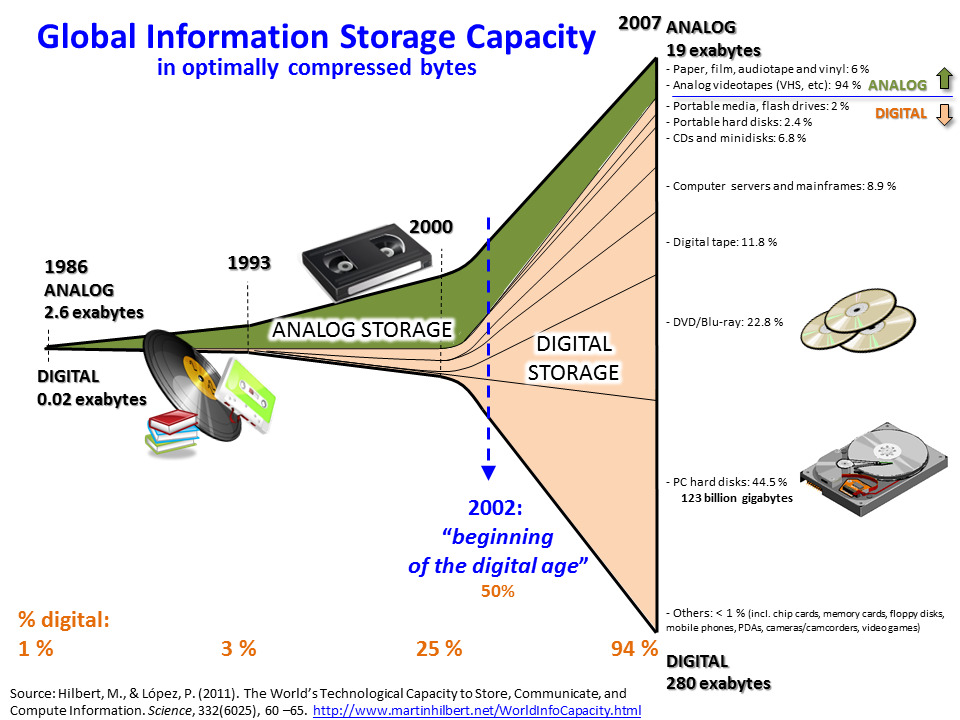
\includegraphics[width=1\linewidth]{images/datarevolution} 

}

\caption{Datavallankumous (Hilbert, M. ja Lopez, P. (2011) The Worlds Technological Capacity to Store, Communicate and Compute Information. Science, 332(6025), 60-65.}\label{fig:datarevolution}
\end{figure}

\begin{itemize}
\tightlist
\item
  ``Danger zone''

  \begin{itemize}
  \tightlist
  \item
    Kuvan \ref{fig:datasc} ``danger zone'' (\href{https://duchesnay.github.io/pystatsml/introduction/machine_learning.html}{Duchesnay, 2020}) kuvaaa tilannetta, jossa ilmiöiden/mallien tilastotieteellinen perusta unohdetaan.
  \item
    Tilastotieteen näkökulman ohittava (laiminlyövä) soveltaja ei aina kykene suhtautumaan kriittisesti muodostuvaa ennustemallia, tai ennustetulosta, kohtaan eikä täten päädy parhaisiin mahdollisiin (tarkimpiin) ennustetuloksiin tilanteessa, jossa jokin toinen malli kuvaisi ilmiötä annettua mallia paremmin.
  \item
    Ko. soveltaja ottaa mallin sekä sen antaman ennustetuloksen annettuna, eikä mieti \emph{mistä kyseinen ennustetulos johtuu}. Jotta tarkat ennustetulokset toteutuvat jatkossakin (kun uutta aineistoa, dataa, tulee saataville), on ennustajan oleellista huomioida mitkä tekijät johtivat tarkkaan ennustulokseen.
  \item
    Eri menetelmät sopivat eri sovelluskohteisiin. Tilastotieteilijä osaa useimmiten tunnistaa eri sovelluskohteisiin sopivat menetelmät paremmin kuin tietojenkäsittelijä. Vastaavasti tehokkaan/onnistuneen ohjelmointikoodin kirjoittamisessa tilanne on usein toisinpäin.
  \end{itemize}
\end{itemize}

\hypertarget{alaluku34}{%
\section{Tilastotieteen osa-alueet}\label{alaluku34}}

\begin{itemize}
\tightlist
\item
  Tilastotiede on saanut alkunsa siitä, että yhteiskunnan modernisoituessa on tarvittu yhä enemmän tietoja erilaisiin hallinnollisiin tarpeisiin. Samalla on syntynyt tarve kehittää menetelmiä joiden avulla tilastojen luotettavuutta on voitu parantaa.

  \begin{itemize}
  \tightlist
  \item
    Kehitys oli pitkään ns. ongelmasta menetelmään ja tutkimusalojen erilaisuudesta johtuen myös tilastotiede on kehittynyt vastaamaan monipuolisesti erilaisiin menetelmällisiin ongelmiin!
  \item
    Tämä on johtanut osaltaan siihen, että tilastotiede jakautuu moniin osa-alueisiin. Osa-alueita on niin paljon, että alan huiputkaan eivät voi hallita niitä kaikkia!
  \end{itemize}
\item
  Tästä huolimatta tilastotiede voidaan karkeasti jakaa teoreettiseen ja soveltavaan osa-alueeseen, jotka toimivat alituisessa vuoropuhelussa.
\end{itemize}

\textbf{Soveltava tilastotiede}

\begin{defblock}{}
\textbf{Soveltava tilastotiede}

on nimensä mukaisesti teoreettisen tilastotieteen kehittämien menetelmien soveltamista jonkin tutkimusalan empiiriseen ongelmaan. Suurin osa tilastotieteen menetelmistä on alun perin kehitetty jonkin konkreettisen tutkimusongelman innoittamana.

\end{defblock}

\begin{itemize}
\tightlist
\item
  Yleisesti ottaen eri tieteenaloilla kohdattavat menetelmäsuuntaukset voidaan jakaa kahteen luokkaan tutkimusaineistojen tyypin perusteella:

  \begin{itemize}
  \tightlist
  \item
    \textbf{Kvantitatiivinen}: eli määrällinen tutkimus on tutkimusta, jossa tutkimusongelma on muotoiltu tarkasti etukäteen ja tutkimuskysymyksiin vastataan käyttäen tilastollisia menetelmiä pyrkien \textbf{selittämään ja ennustamaan} tutkimuksen kohteena olevaa ilmiötä.

    \begin{itemize}
    \tightlist
    \item
      Täsmällisten ja laskennallisten tilastollisten menetelmien käyttäminen numeeriseen aineistoon on kvantitatiiviselle tutkimukselle ominaisin piirre.
    \item
      Perustuu yleensä satunnaisotokseen (kts. luvut \ref{luku4}, \ref{luku5} ja \ref{luku6}) ja tutkimusaineisto on tiivistetty numeeriseksi havaintomatriisiksi, jolle oleellinen vaatimus on sen totuudellisuus.
    \item
      \textbf{Kritiikki}: määrällinen tutkimus on (paikoin) sokea tutkittavien ilmiöiden sellaiselle luonteelle, jota ei pystytä kvantifioimaan, eli muuntamaan numeeriseen muotoon. Näihin voidaan katsoa lukeutuvan mm. tunteet, merkitykset ja kokemukset, ellei tutkija keksi niiden numeeriselle mittaamiselle uskottavaa keinoa.\\
    \end{itemize}
  \item
    \textbf{Kvalitatiivinen}: eli laadullinen tutkimus on tutkimusta, jossa tutkimuksen kohteena olevaa ilmiötä ja sen merkitystä sekä tarkoitusta pyritään \textbf{ymmärtämään} kokonaisvaltaisella tavalla.

    \begin{itemize}
    \tightlist
    \item
      Laadullisessa tutkimuksessa annetaan usein tilaa tutkimuksen kohteena olevien ilmiöiden ja/tai ihmisten näkökulmille, vaikuttimille, kokemuksille ja tuntemuksille. Tutkimusyksikköjen otanta on täten usein harkinnanvaraista.
    \item
      Laadullisessa tutkimuksessa tutkimusongelma muotoutuu tutkimuksen edetessä ja sille tyypillistä on hypoteesittomuus, eli tutkimus on tarkoitus aloittaa mahdollisimman vähin ennakko-oletuksin. Ennakko-oletuksista on kuitenkin mahdotonta täysin irtautua, joten niiden ilmi tuominen esioletuksina tai ``tutkimushypoteeseina'' eli arvauksina tuloksista on osa tutkimusta.
    \item
      Kritiikkiä: laadullinen tutkimus ei pysty vastaamaan kysymykseen miksi, sillä ilman määrällisiä (numeraalisia) aineistoja ei ilmiöiden välisiä riippuvuuksia kyetä tutkimaan: \textbf{laadullisessa tutkimuksessa menetetäänkin mahdollisuus tutkia ilmiöiden todellisia syitä}.

      \begin{itemize}
      \tightlist
      \item
        Laadullinen tutkimus nähdään usein vähemmän objektiivisena ja sen otosta koskevia tuloksia ei useinkaan voida yleistää koskemaan perusjoukkoa.
      \end{itemize}
    \end{itemize}
  \end{itemize}
\end{itemize}

\hfill\break
\hfill\break

\begin{itemize}
\tightlist
\item
  \textbf{Yleisenä menetelmätieteenä tilastotiedettä voidaan (ja myös pitäisi) soveltaa kaikilla reaalimaailmaa tutkivilla tieteenaloilla, joiden tutkimusaineistot voidaan esittää kvantitatiivisessa muodossa.}

  \begin{itemize}
  \tightlist
  \item
    Tilastollisten menetelmien käyttö on siis huomattavan paljon yleisempää määrällisessä kuin laadullisessa tutkimuksessa.
  \end{itemize}
\item
  Menetelmien soveltamisen tarkoituksena on (voi olla):
  \textbf{i)} \textbf{kuvailla ja tiivistää tietoa}, jota havaittu aineisto sisältää
  \textbf{ii)} sovellusalan oman \textbf{teorian empiirinen testaus} tai
  \textbf{iii)} edellisten pohjalta tehtävä \textbf{tilastollinen päättely}.

  \begin{itemize}
  \tightlist
  \item
    \textbf{Deskriptiivisellä eli kuvailevalla tilastotieteellä} tarkoitetaan sellaisten menetelmien soveltamista, joiden avulla havaintoaineistosta voidaan esimerkiksi laskea tunnuslukuja, kuvata havaintomuuttujien jakaumia ja visualisoida aineiston generoimaa ilmiötä tai siitä johdettuja tunnuslukuja.
  \item
    \textbf{Tilastollinen päättely} on sen sijaan aineiston tarkasteluun/kuvailuun sekä mallintamiseen perustuvaa päätöksentekoa, jossa kvantitatiiviseen aineistoon kuuluva epävarmuus ja satunnaisuus on otettu huomioon.

    \begin{itemize}
    \tightlist
    \item
      Keskeinen tilastollisen päättelyn käyttötarkoitus soveltajille on usein \textbf{teorian ja siihen liitettävien hypoteesien testaaminen}, joka voi johtaa joko teorian vahvistumiseen (\emph{verifiointiin}) tai sen vääräksi osoittamiseen (\emph{falsifioimiseen}) (ks. luku \ref{alaluku21}).
    \item
      On myös syytä muistaa, että yksi tutkimus ei vielä osoita teoriaa oikeaksi tai vääräksi vaan siihen tarvitaan useita tutkimuksia sekä erilaisia tutkimusasetelmia ja -menetelmiä.
    \end{itemize}
  \item
    Kuvaileva tilastotiede ja tilastollinen päättely kulkevat soveltavassa tilastollisessa tutkimuksessa käsi kädessä.
  \end{itemize}
\end{itemize}

\begin{figure}

{\centering 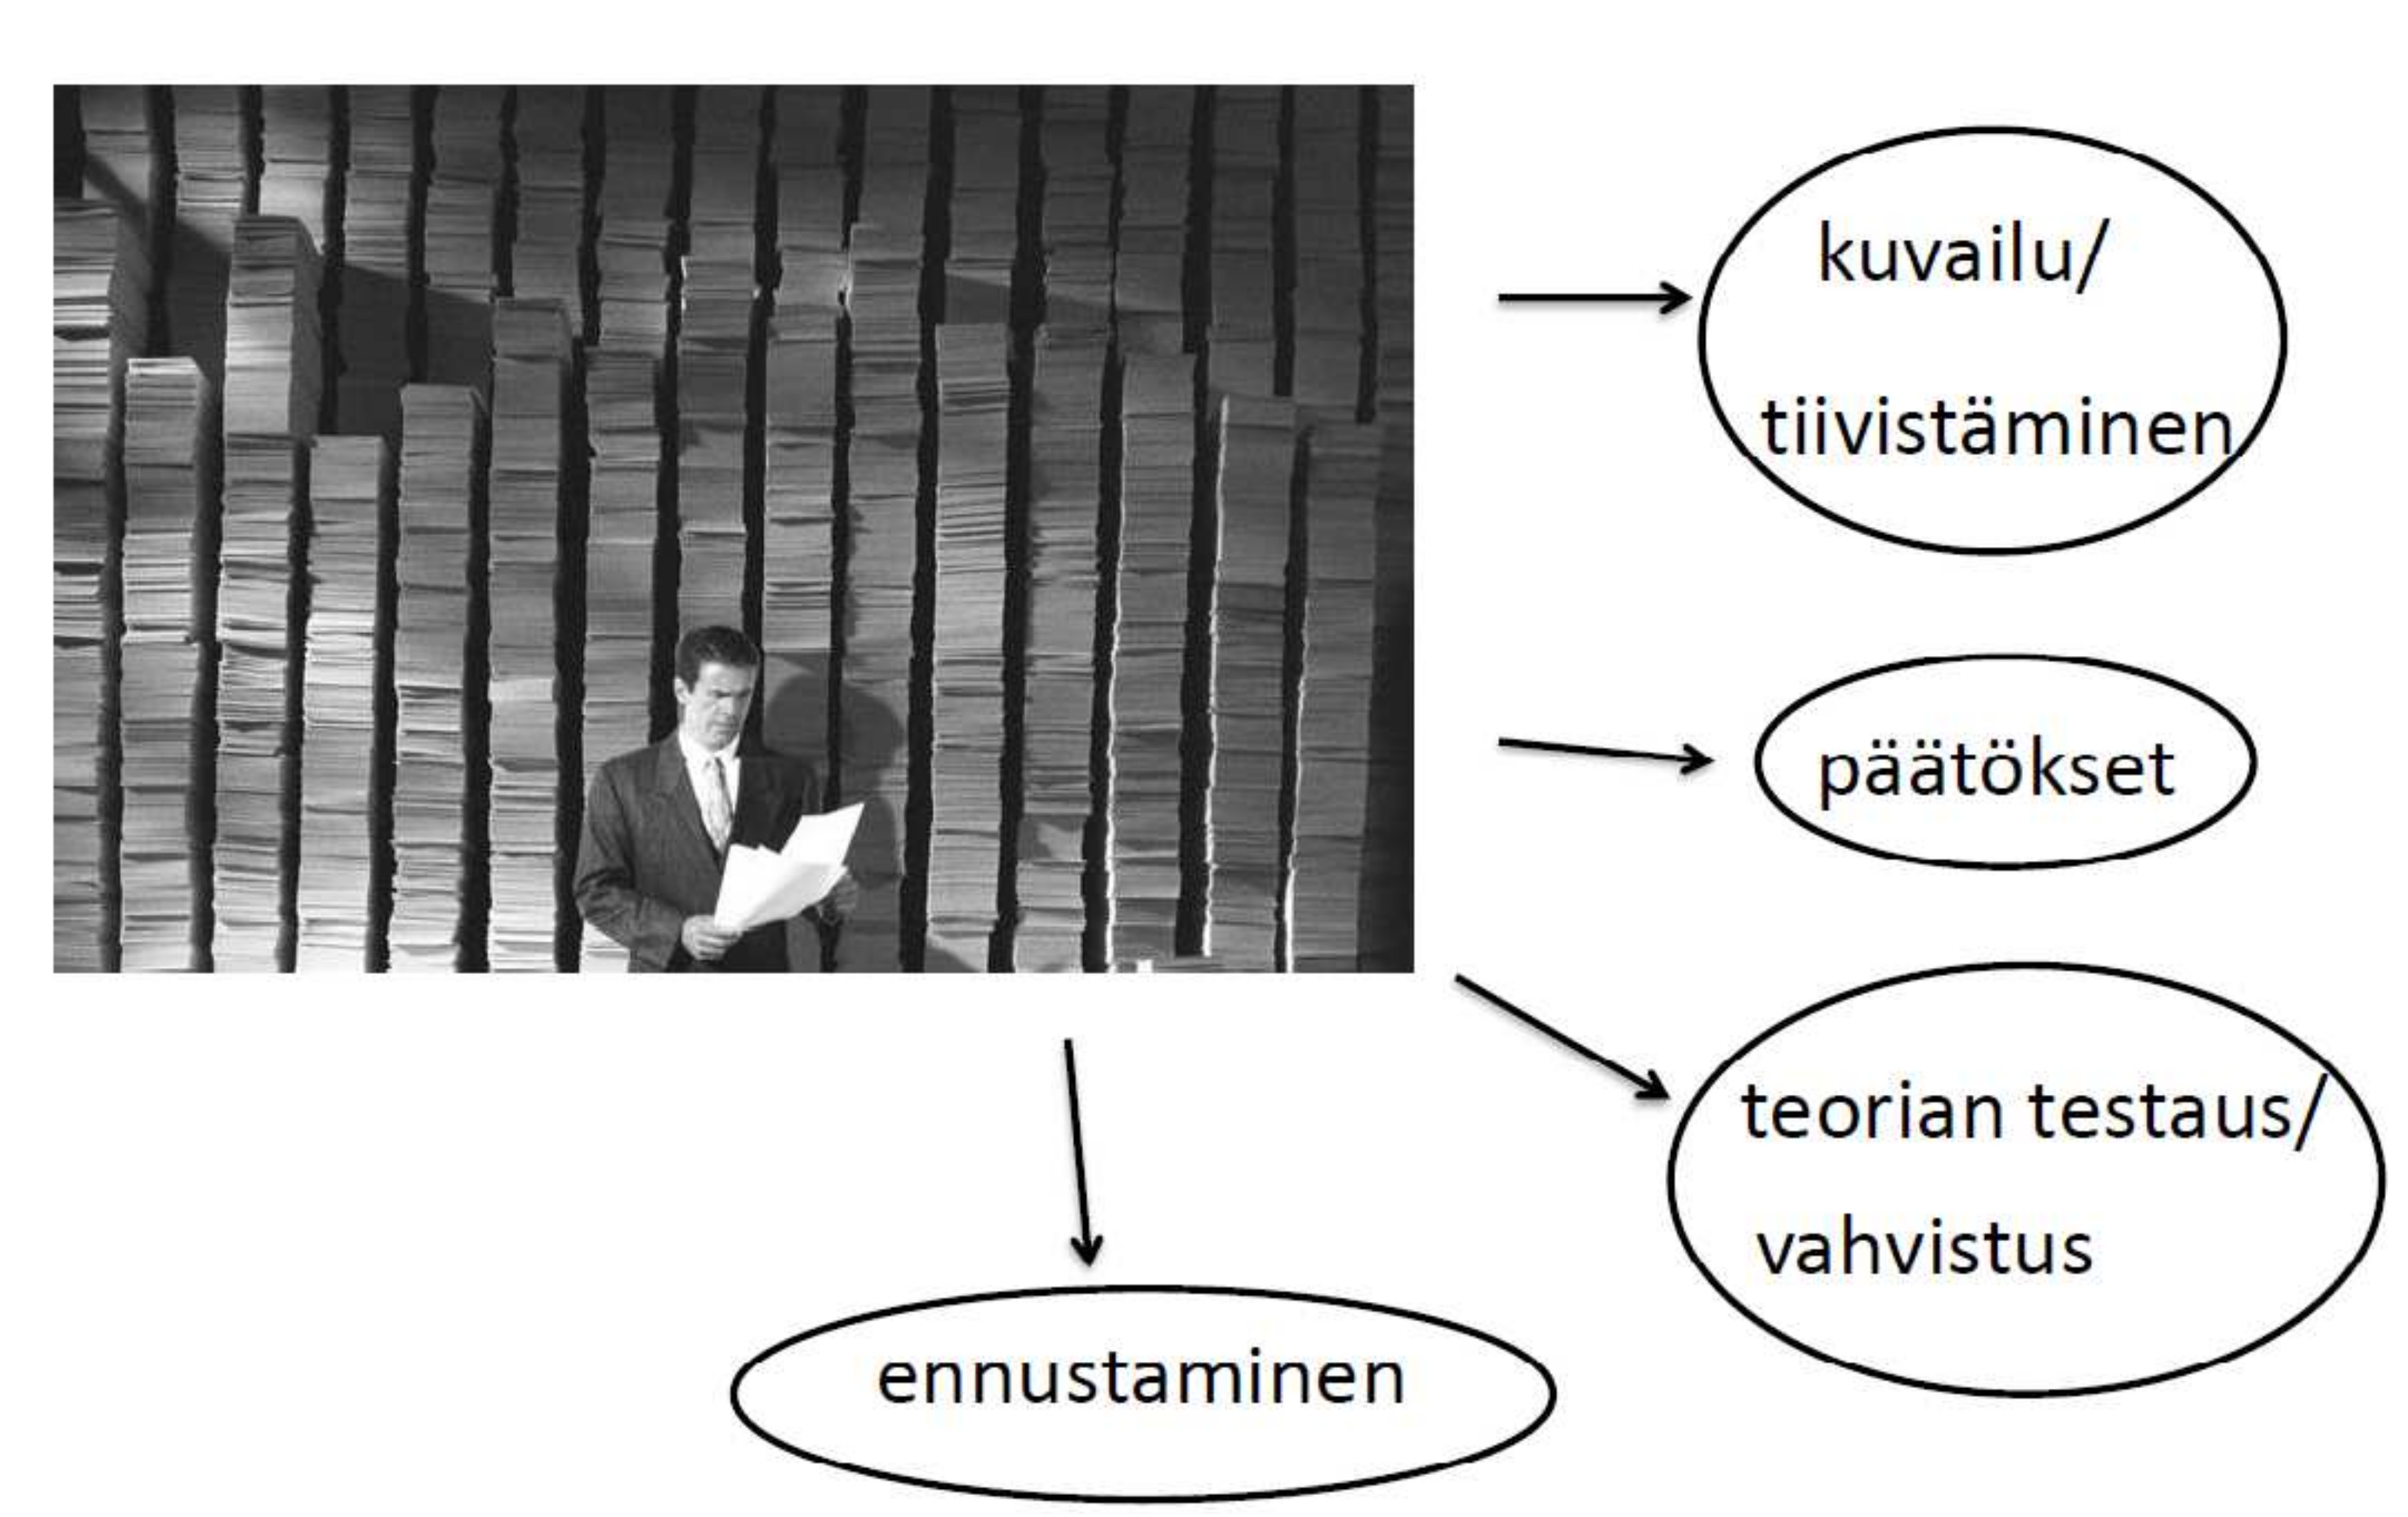
\includegraphics[width=1.5\linewidth]{images/soveltava} 

}

\caption{Soveltava tilastotiede}\label{fig:soveltava}
\end{figure}

\hfill\break
\hfill\break

\textbf{Teoreettinen tilastotiede}

\begin{defblock}{}
\textbf{Teoreettinen tilastotiede} kehittää (tilasto)matemaattisia malleja kuvaamaan satunnaisilmiöitä- ja prosesseja, jotka generoivat reaalimaailman ilmiöitä kuvaavia numeerisia tai kvantitatiivisia tietoja, joihin liittyy epävarmuutta ja satunnaisuutta.

\end{defblock}

\begin{itemize}
\tightlist
\item
  Teoreettinen tilastotiede luo pohjan tilastollisten menetelmien ymmärtämiselle, soveltamiselle ja kehittämiselle.

  \begin{itemize}
  \tightlist
  \item
    Ilman riittävää ymmärrystä tilastollisten menetelmien toimintaperiaatteista niiden soveltaja on vaarassa tehdä virhepäätelmiä! (Ks. alaluku \ref{alaluku35} tilastotieteen kritiikistä)
  \end{itemize}
\item
  Mallit perustuvat todennäköisyyslaskentaan, ja niitä kutsutaan tilastollisiksi malleiksi, stokastisiksi malleiksi tai todennäköisyysmalleiksi.

  \begin{itemize}
  \tightlist
  \item
    Tilastolliset mallit perustuvat laajalti niin kutsuttuun uskottavuusfunktioon. Se on malli, joka riippuu havaintoaineiston lisäksi yhdestä tai useammasta parametrista. (ks. tarkemmin luku \ref{luku6})
  \item
    Uskottavuusfunktion arvo kertoo kuinka todennäköisenä voidaan havaittua aineistoa pitää, mikäli sen oletetaan olevan peräisin vastaavasta mallista jollain parametriarvoilla.
  \item
    Uskottavuuspäättelyn perusajatuksena on, että se tai ne parametriarvot, joilla uskottavuusfunktion arvo maksimoituu kuvaa aineiston generoinutta prosessia parhaiten.
  \item
    Aineistoa koskevia hypoteeseja voidaan testata käyttäen uskottavuusfunktion maksimia vastaavaa tilastollista mallia!
  \item
    \emph{``Kaikki mallit ovat vääriä, mutta jotkut ovat käyttökelpoisia.''} (Box, 1976).
  \end{itemize}
\end{itemize}

\hfill\break
\hfill\break

\begin{itemize}
\tightlist
\item
  Uskottavuusfunktiot perustuvat aina satunnaisilmiöiden mahdollisia arvoja kuvaaviin nk. \textbf{tiheysfunktioihin} tai todennäköisyysfunktioihin.

  \begin{itemize}
  \tightlist
  \item
    Tiheysfunktiot kuvaavat jonkin satunnaismuuttujan (satunnaisilmiön) saamien arvojen jakaumaa.
  \item
    Esimerkiksi kolikonheitto on satunnaisilmiö ja sillä on vain kaksi arvoa\footnote{Kolikon kantilleen jäämistä ei tässä lasketa mahdolliseksi tapahtumaksi.} ja kolikonheittoa voidaan kuvata nk. binomijakaumalla, merkitään \(\text{Bin}(n,p)\) missä \(n\) on heittojen lukumäärä ja \(p\) on kruunan todennäköisyys.
  \item
    Esimerkki: heitetään kolikkoa 40 kertaa ja saadaan kruuna 40/40 tapauksessa. Onko tämän havaintoaineiston perusteella uskottavaa, että kolikonheitto noudattaa binomijakaumaa \(\text{Bin}(40, 0.5)\)? Eli kuinka uskottavan voidaan pitää että kyseinen kolikko on tavallinen, painottamaton kolikko?
  \end{itemize}
\end{itemize}

\begin{figure}

{\centering 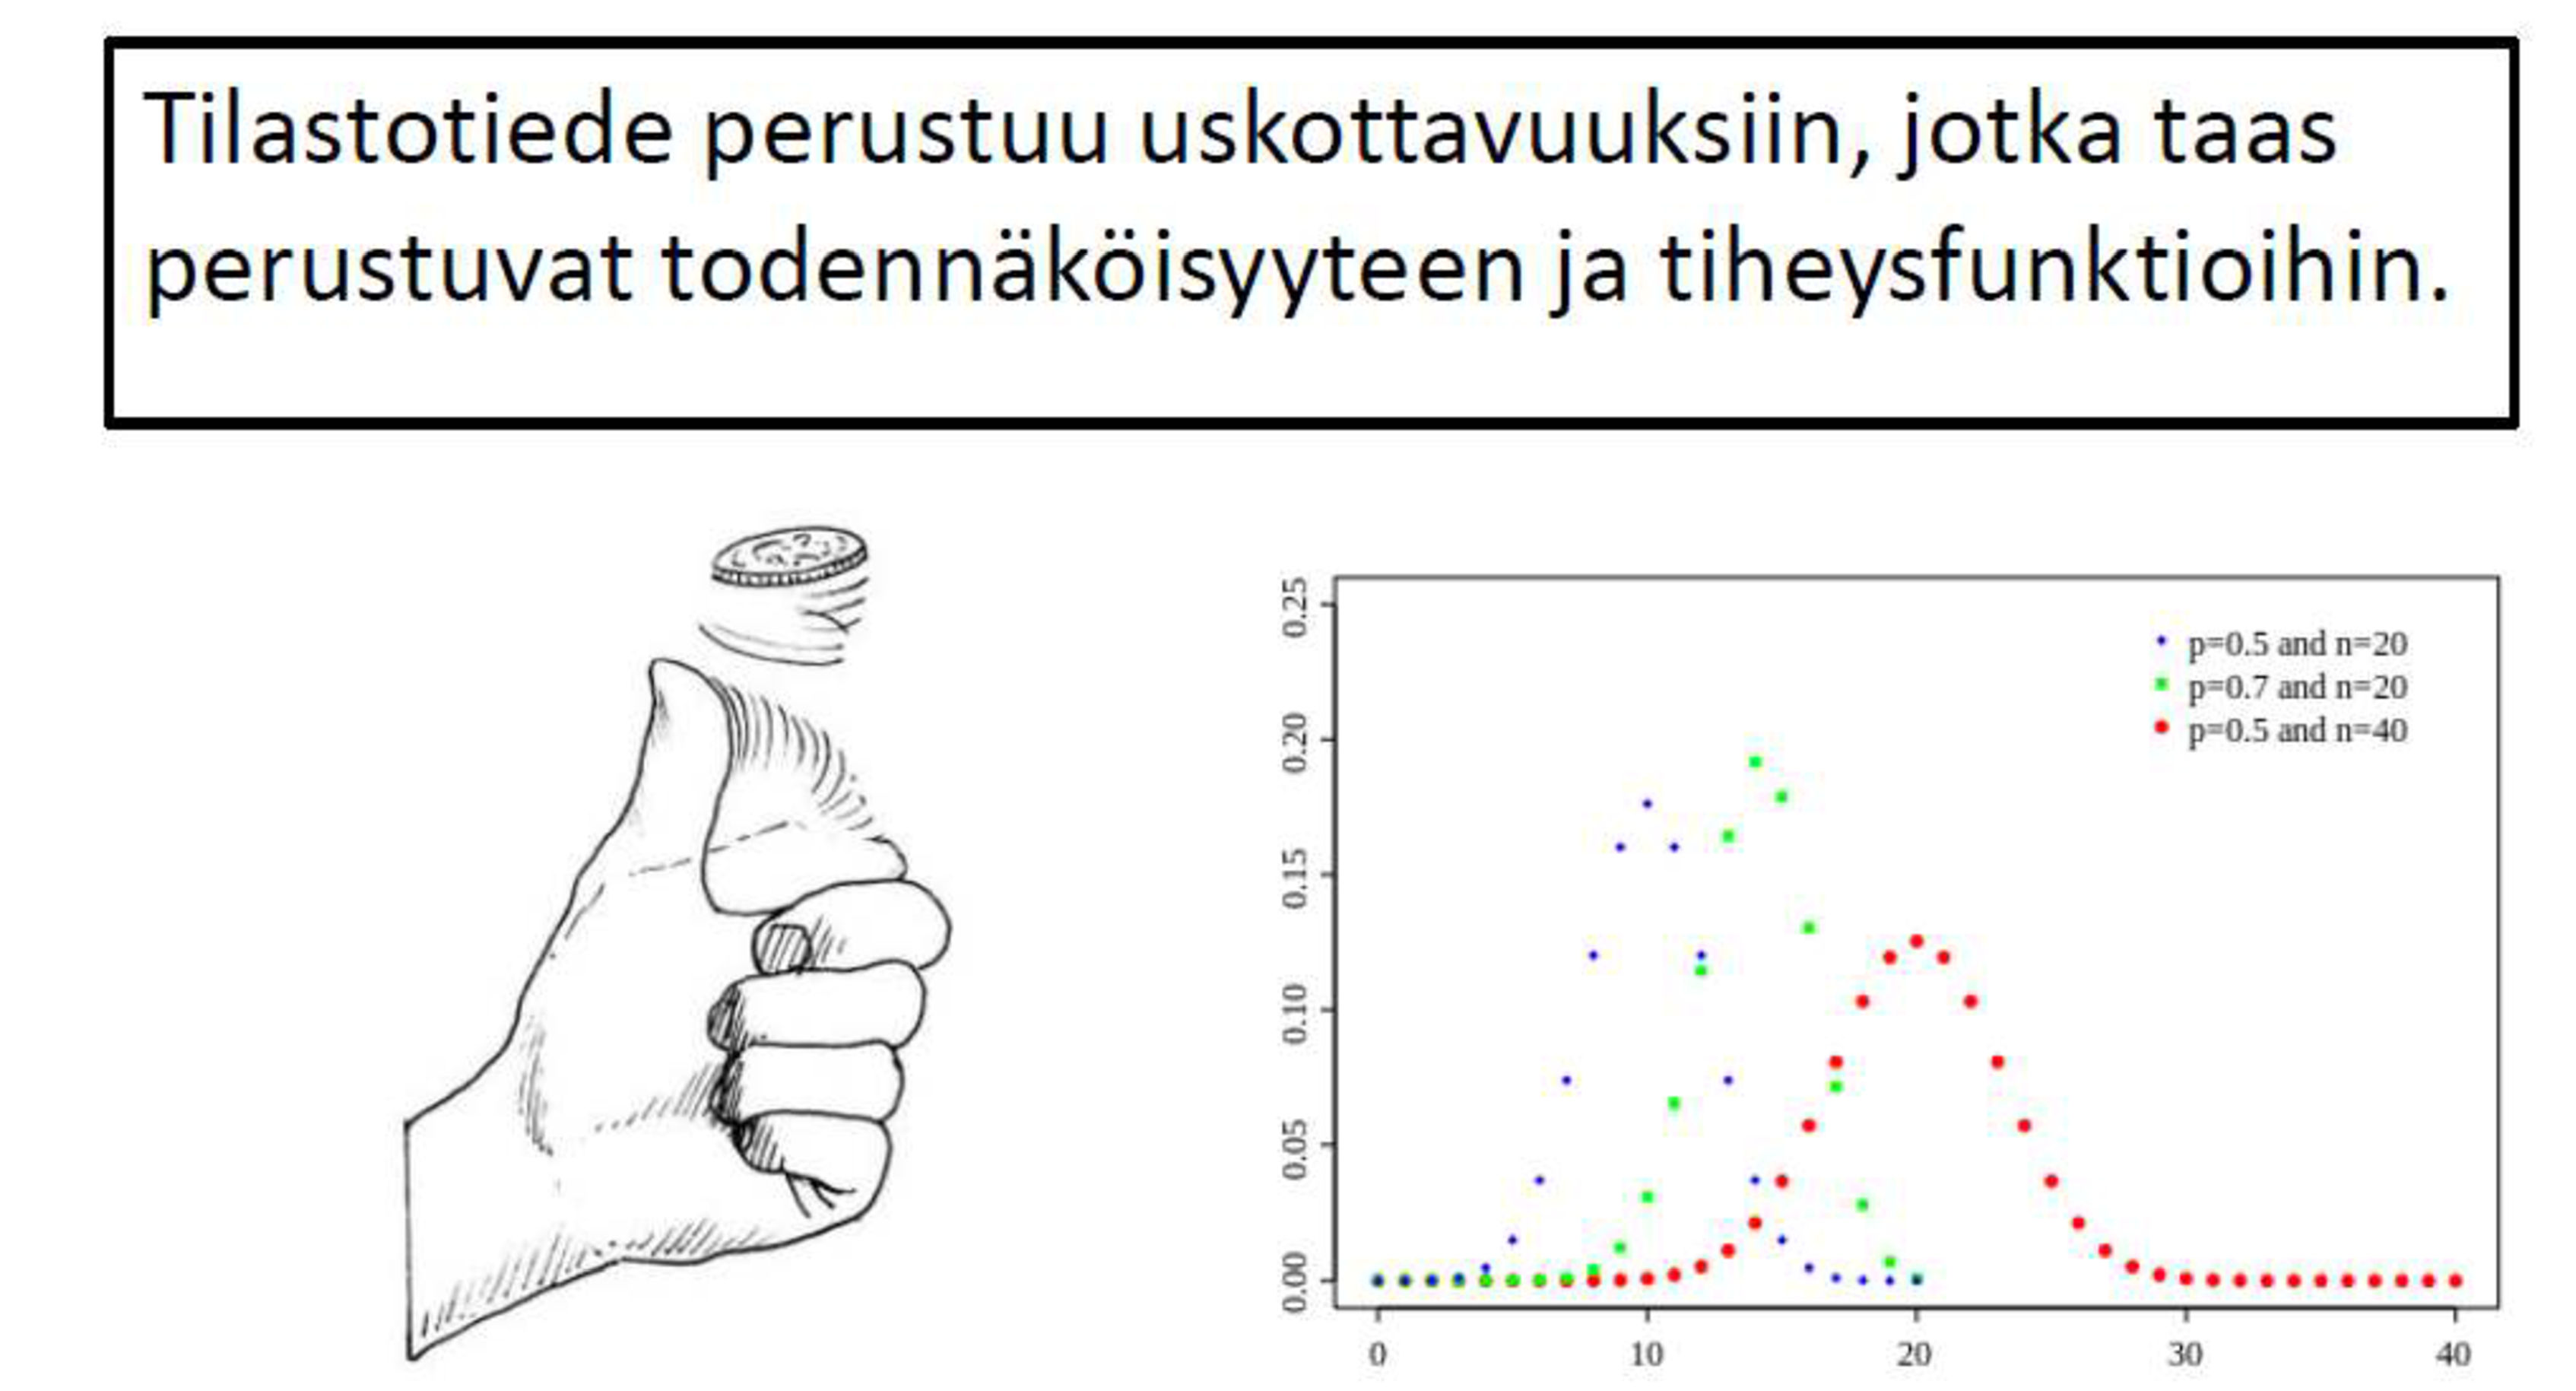
\includegraphics[width=1.5\linewidth]{images/perustuu} 

}

\caption{Tilastotiede ja todennäköisyys}\label{fig:perus}
\end{figure}

\hfill\break
\hfill\break

\begin{itemize}
\tightlist
\item
  Todennäköisyyslaskenta luo tilastotieteelliselle epävarmuuden mallintamiselle vahvan ja uskottavan matemaattisen perustan.

  \begin{itemize}
  \tightlist
  \item
    Todennäköisyyslaskentaa opetetaan tarkemmin (tätä kurssia seuraavilla) kursseilla \href{https://opas.peppi.utu.fi/fi/opintojakso/TILM3553/1734}{TILM3553 Todennäköisyyslaskennan peruskurssi pääaineopiskelijoille}, \href{https://opas.peppi.utu.fi/fi/opintojakso/TILM3568/3385}{TILM3568 Todennäköisyyslaskenta sivuaineopiskelijoille} ja \href{https://opas.peppi.utu.fi/fi/opintojakso/SMAT5306/4400}{SMAT5306 Todennäköisyyslaskennan jatkokurssi}.
  \end{itemize}
\end{itemize}

\begin{figure}

{\centering 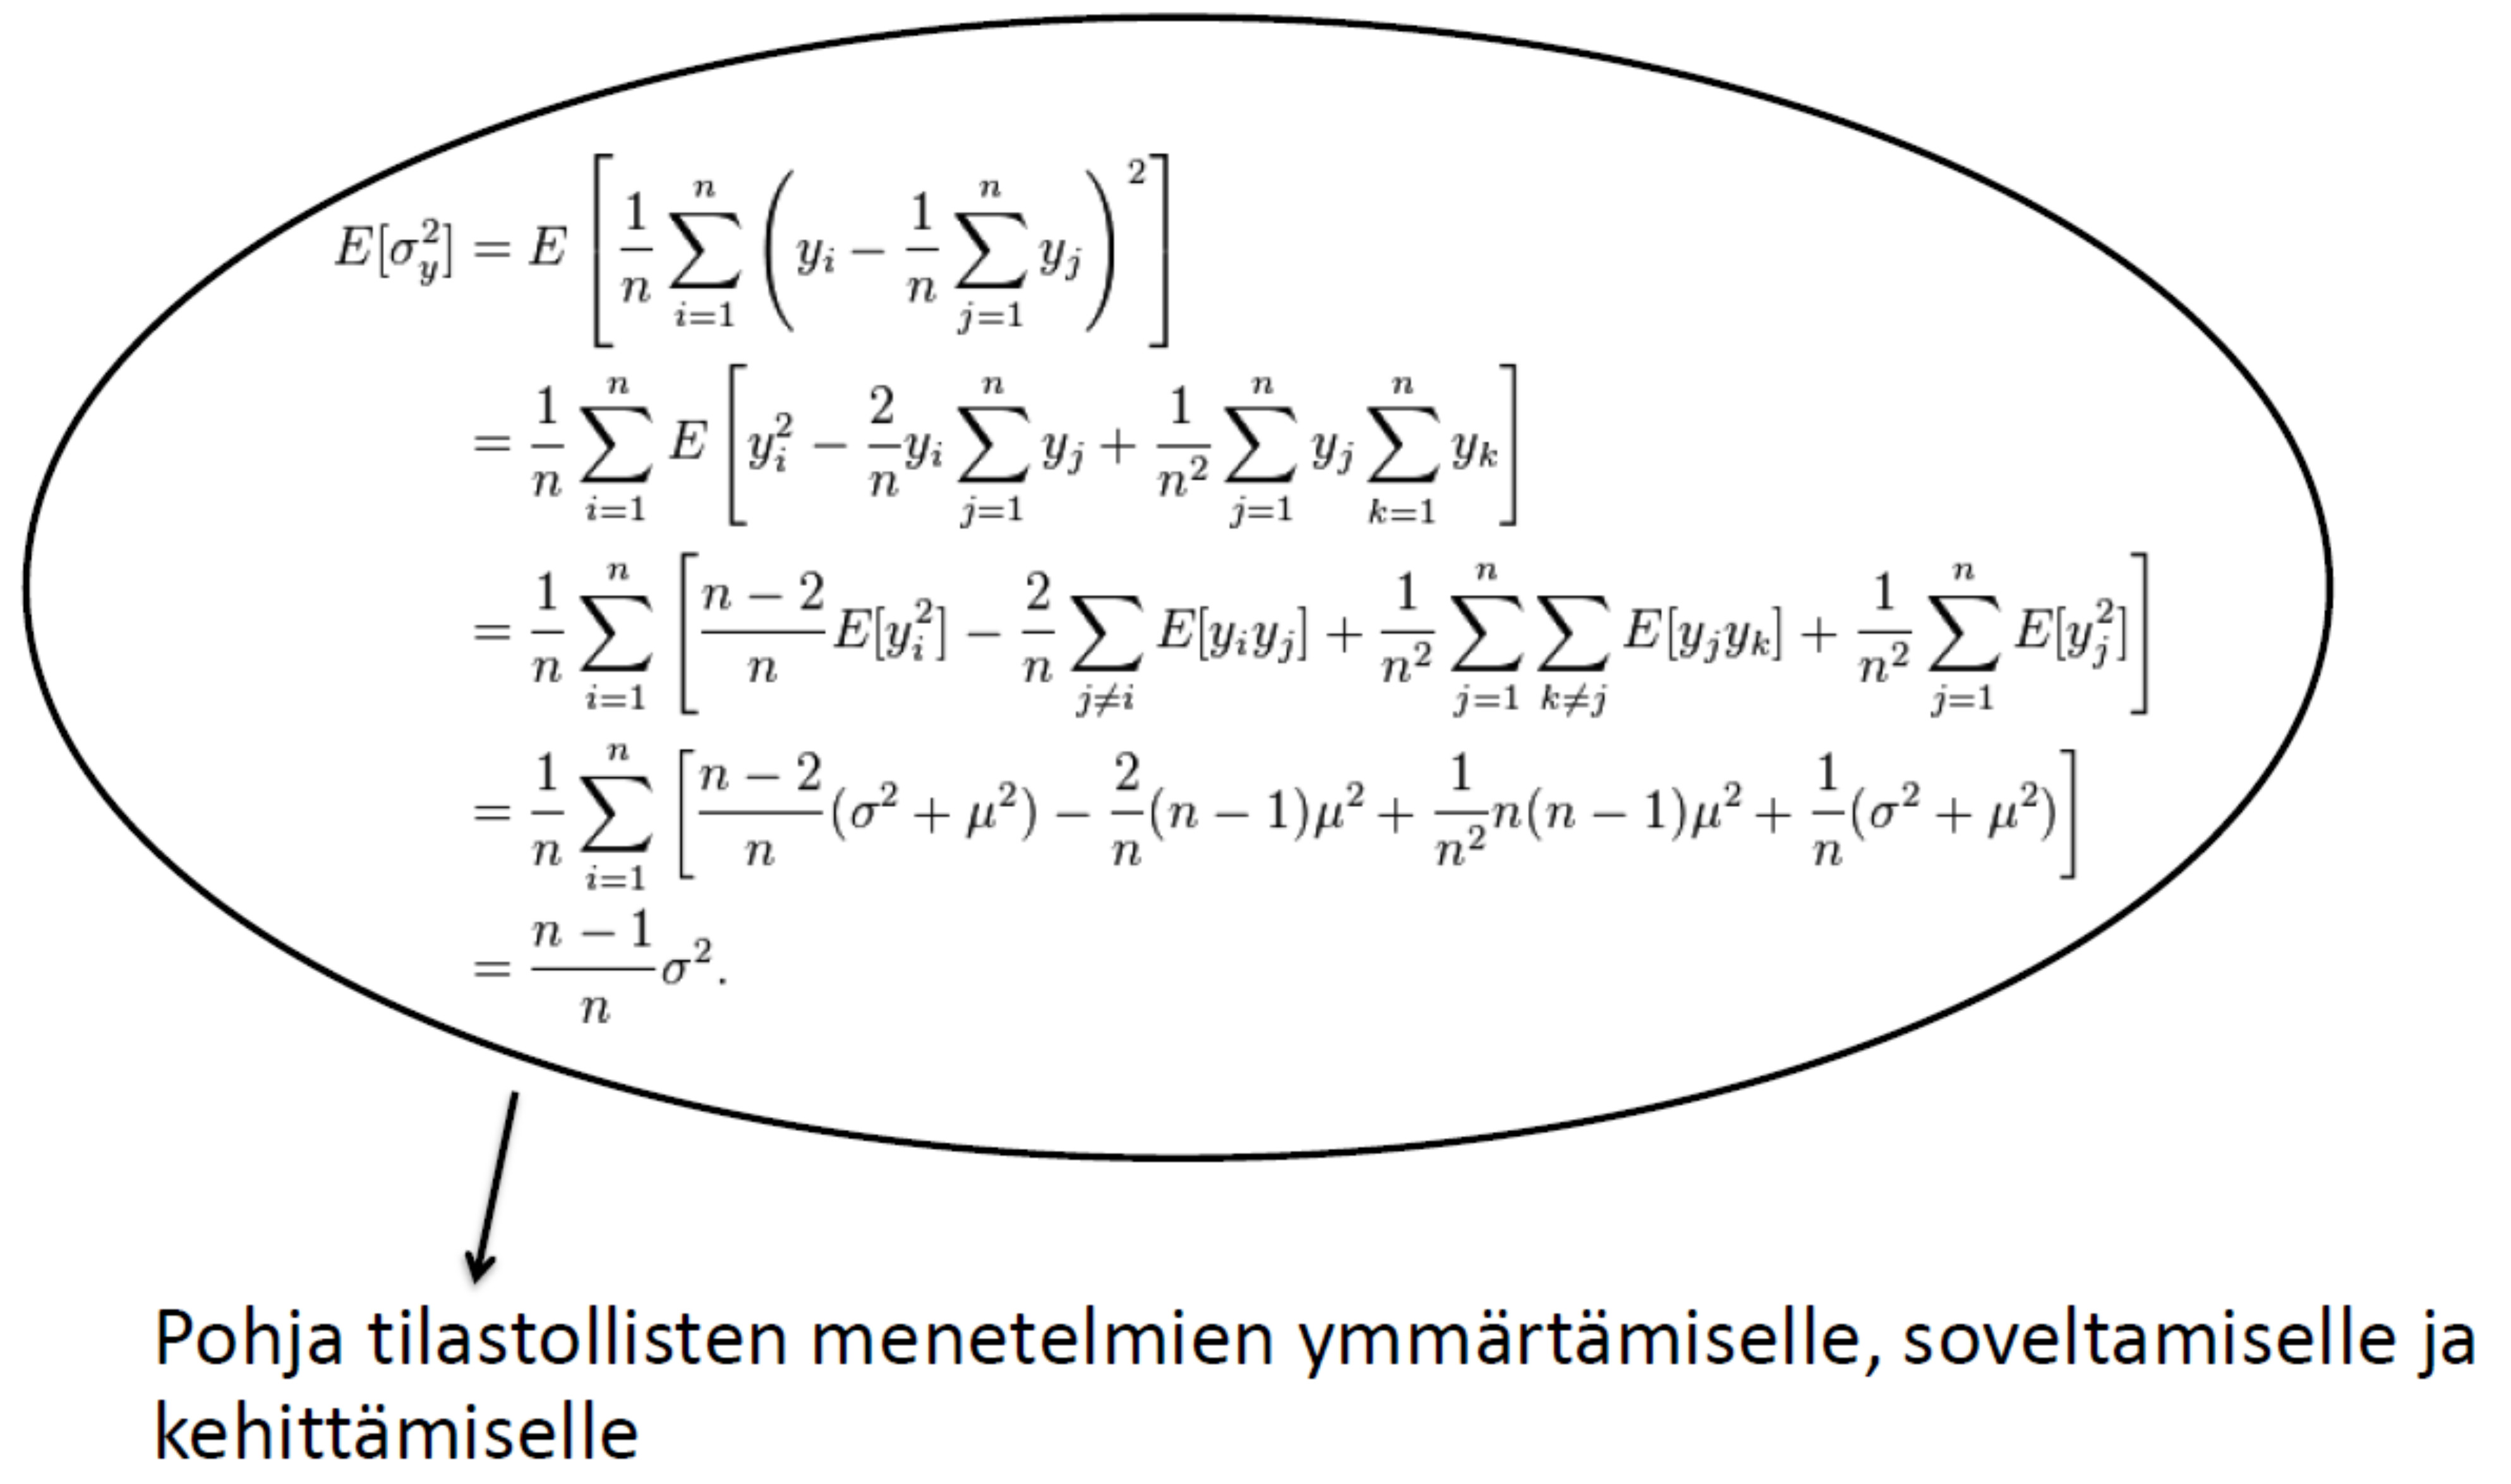
\includegraphics[width=1.5\linewidth]{images/teoreettinen} 

}

\caption{Teoreettinen tilastotiede}\label{fig:teoreettinen}
\end{figure}

\hypertarget{alaluku35}{%
\section{Tilastotieteen kritiikkiä}\label{alaluku35}}

\begin{itemize}
\tightlist
\item
  Tilastotieteen rooli tiedeyhteisössä on niin tärkeä että sitä kohtaan on ymmärrettävästi esitetty myös paljon kritiikkiä. Valtaosa kritiikistä kohdistuu joko tilastotieteen matemaattisuuteen tai sitten siinä tarvittaviin oletuksiin, jotka mahdollistavat esimerkiksi hypoteesien testaamisen.

  \begin{itemize}
  \tightlist
  \item
    Usein kritiikki on aiheetonta ja johtuu sen esittäjän puutteellisesta tilastotieteen ymmärryksestä. Perusteettoman kritiikin esittäminen toista tieteenalaa kohtaa ei kuitenkaan ole vieras ilmiö juuri millään alalla.
  \end{itemize}
\item
  Tässä alaluvussa käymme läpi yleisimpiä kritiikin muotoja, joita tilastotiedettä kohtaan esitetään ja pyrimme tarjoamaan vastauksia/vastineita silloin kun niitä voidaan antaa.
\end{itemize}

\hfill\break
\hfill\break

\textbf{``Yleismaailmallinen'' kritiikki}

\begin{itemize}
\tightlist
\item
  Aloitetaan yleismaailmallisella kritiikillä, jota tilastollista tutkimusta vastaan on esitetty:

  \begin{itemize}
  \tightlist
  \item
    Tilastotieteessä käytettävien tunnuslukujen, kuten keskiarvon, reaalimaailman vastineet ovat joskus mielivaltaisia. Esimerkiksi keskiarvo on ajoittain ongelmallinen tunnusluku, sillä lienee varsin selvää, että keskimääräistä ihmistä ei ole olemassa vaikka tilastotieteessä näitä tunnuslukuja usein lasketaankin.

    \begin{itemize}
    \tightlist
    \item
      Esimerkiksi puhekielessä yleinen nk. ``Keskiarvo-Kalle'', eli 1,8 lapsen vanhempi ja 1,5 auton omistaja on tietenkin täysin kuvitteellinen.
    \item
      Lisäksi joskus kuulee tilastotieteilijöitä kritisoitavan lausumalla ``\emph{Jos toinen jalka on jääkylmässä vedessä ja toinen kiehuvassa vedessä, niin tilastotieteilijän mielestä ihmisellä on tällöin keskimäärin hyvä olla}''
    \end{itemize}
  \end{itemize}
\item
  Korrelaatio on tunnusluku, joka kuvaa kahden muuttujan välistä riippuvuutta (palaamme tähän tarkemmin luvussa \ref{luku7}). Se ei kuitenkaan kuvaa millään tavoin kausaalisuutta, eli sitä kumpi aiheuttaa kumman, jos kumpikaan.\footnote{Tyler Vigen on kerännyt verkkosivuilleen}(\url{https://www.tylervigen.com/spurious-correlations}) mitä moninaisimpia esimerkkejä kahdenvälisistä nk. \emph{näennäisistä} korrelaatioista.

  \begin{itemize}
  \tightlist
  \item
    Esimerkiksi ``jäätelön syönti ja hukkumiskuolemat'' -tapauksessa havainnollisesti todetaan jäätelönkulutuksen ja hukkumiskuolemien lukumäärän korreloivan keskenään, mutta taustalla vaikuttava tekijä onkin lämmin kesä, joka vaikuttaa molempiin.
  \end{itemize}
\item
  Vaikkei näiden esimerkkien oikeellisuutta ole syytä kiistää, niin tilastollisen tiedon arvioinnissa on kuitenkin syytä päästä syvemmälle.
\end{itemize}

\hfill\break
\hfill\break

\textbf{Kritiikki matemaattisuutta kohtaan}

\begin{itemize}
\tightlist
\item
  Ehkä merkittävin kritiikki tilastollisia menetelmiä kohtaan kohdistuu kritiikin näkökulmasta perusteettomaan, tai ainakin liian vahvaan, matemaattisuuden tuomaan itsevarmuuteen. Voidaankin siis perustellusti kysyä, että \textbf{onko tieteellisyys = matemaattisuus}?

  \begin{itemize}
  \tightlist
  \item
    Useat tieteenalat käyttävät tutkimuksessaan edistyneitäkin tilastollisia menetelmiä siitä huolimatta, että tutkijoiden tilastomatemaattinen pohjakoulutus ei välttämättä ole riittävällä tasolla kyseisten menetelmien kokonaisvaltaiseen ymmärtämiseen.

    \begin{itemize}
    \tightlist
    \item
      Helppokäyttöisistä tilasto-ohjelmistoista on riittävät perustaidot omaaville käyttäjille erittäin paljon hyötyä mutta koneiden ja ohjelmien käytön opettelu ei kuitenkaan ole varsinaista tilastotiedettä (tarvitaan enemmän tilastotieteen opintoja).
    \item
      Laskentatehon ja modernin tietojenkäsittelyteknologian ansiosta monimutkaisiakin tilastollisia analyysejä on kuitenkin mahdollista tehdä vaikka tutkijalla olisi tilastotieteestä vain perustiedot, jos sitäkään.
    \item
      Pahimmillaan tämä saattaa johtaa siihen, että analyyseja tehdään ymmärtämättä mitä itse asiassa ollaan tekemässä.
    \end{itemize}
  \item
    Tilastollisten analyysien hyödyllisyyden ja järkevyyden ehtona on kuitenkin käytettävien menetelmien, aineiston ja tutkittavan ilmiön pintaa syvemmälle ulottuva tuntemus.

    \begin{itemize}
    \tightlist
    \item
      Käytettävien tilastollisten menetelmien oletukset on osattava ottaa huomioon ja toisaalta odottamattomien tulosten syyt on pystyttävä jäljittämään.

      \begin{itemize}
      \tightlist
      \item
        Teknistä esitystä käyttävää tutkijaa saatetaan pitää erityisen uskottavana, koska hän kykenee käyttämään vaikeita menetelmiä. Tästä huolimatta tutkimusongelma ei saisi päästä unohtumaan.
      \item
        Tutkijan tulisikin varmistua siitä, että käytettävät menetelmät todella vastaavat asetettuihin tutkimuskysymyksiin ja että tutkimusongelma on ratkaistavissa käytettävillä menetelmillä.
      \item
        Tekninen esitys ei takaa onnistunutta tilastollista tutkimusta eri näkökulmista katsoen. Monet tilastolliset menetelmät ovat vaikeita ja vaativat soveltajiltaan paljon.
      \item
        Lisäksi on hyvä muistaa, että käytettävien menetelmien lähtökohdat ja oletukset eivät matemaattisuudestaan huolimatta ole välttämättä neutraaleja!
      \end{itemize}
    \item
      Kaikkia tieteentekijöitä ei voida velvoittaa opiskelemaan edistynyttä abstraktia tilastotieteen teoriaa (tilastomatematiikkaa), mutta menetelmien oikeaoppinen käyttö kuitenkin vaatii riittävää ymmärrystä.
    \end{itemize}
  \end{itemize}
\end{itemize}

\hfill\break
\hfill\break

\textbf{Kritiikki yksinkertaistuksia kohtaan}

\begin{itemize}
\tightlist
\item
  Edellisiä kohtia yleisemmin tilastotiedettä on kritisoitu siitä, että se ei kykene riittävällä tasolla huomioimaan reaalimaailman kompleksisuutta.

  \begin{itemize}
  \tightlist
  \item
    Merkittävässä osassa tilastollisia analyyseja lähtökohtana on usko ``todellisen'' maailman ja näin ollen aineistoa generoivien mekanismien olemassaoloon.

    \begin{itemize}
    \tightlist
    \item
      Tätä saatetaan usein pitää kuitenkin kyseenalaisena: voiko ``tosielämän stokastiikasta'' muka todella löytyä säännönmukaisuuksia?
    \item
      Tämä kysymys on kuitenkin pitkälti tieteenfilosofinen ja palautuu lopulta sovellusalaan sekä tutkimusongelmaan ja -kysymykseen: tilastollisten menetelmien toimivuutta voidaan helposti testata esimerkiksi simulaatiokokeilla.\\
    \end{itemize}
  \item
    Tilastotiedettä on myös kritisoitu sen ``sokeudesta'' sosiaaliseen vuorovaikutukseen liittyviin subjektiivisiin kokemuksiin kuten tunteisiin, kokemuksiin ja ei-numeeriisiin havaintoihin.

    \begin{itemize}
    \tightlist
    \item
      Tämä kritiikki ei kuitenkaan suoranaisesti ole tilastotieteen kritiikkiä, vaan jälleen sovellusalakohtainen ja erityisesti tutkimuskysymyksen asettelua koskeva ongelma.

      \begin{itemize}
      \tightlist
      \item
        Tuntemuksia ja kokemuksia voidaan hyvin testata tilastollisin menetelmin, mikäli tutkija osaa uskottavasti määritellä niille numeerisen mittauksen kriteeristöt!
      \item
        Tämä on kuitenkin vaikeaa, sillä aivan kaikkea ei voida kvantifioida: kirjoitetun tekstin tai sosiaalisten merkitysten tulkinnan sekä elämysten kuten musiikin ja taiteen aiheuttamien mielikuvien ja tunteiden voidaan perustellusti nähdä olevan hyvin haastavia kvantifioida.
      \end{itemize}
    \item
      Näiden aiheiden tulkinta, ymmärtäminen ja tutkiminen ulottuu kvantitatiivisen tutkimuksen ulkopuolelle.
    \end{itemize}
  \item
    Mikäli tutkittavasta ilmiöstä pystyy kvantitatiivisilla mittauksilla saada relevanttia tietoa, tulisi aineiston analyysin apuna joka tapauksessa aina käyttää tilastollisia menetelmiä!
  \item
    Vaikka kvantitatiivisia aineistoja ei voi pitää objektiivisina faktoina asioiden tilasta, se ei tarkoita, etteivätkö tulokset voisi olla käyttökelpoisia.
  \end{itemize}
\end{itemize}

\hfill\break
\hfill\break

\textbf{Temppukokoelmakritiikki}

\begin{itemize}
\tightlist
\item
  Eräs ehkä osin implisiittinen kritiikki tilastotiedettä kohtaan on sen pitäminen nk. \textbf{``temppukokoelmana''.}

  \begin{itemize}
  \tightlist
  \item
    Tilastotieteen voi nähdä koostuvan numeeristen tietojen jalostamisen menetelmistä. Tämä näkemys, joka on usein tahaton, pelkistää tilastotieteen \emph{vain} \textbf{menetelmäkokoelmaksi}, vailla omaa teoriaa.
  \item
    Eri tutkimusalojen empiirisessä työssä (liian) usein vain kerätään aineisto ja vasta sitten mietitään mitä sillä voitaisiin tehdä.
  \item
    Usein apuun haetaan tilastotieteilijä, jonka odotetaan loihtivan (tilastollisen) ratkaisun ongelmaan kuin ongelmaan.

    \begin{itemize}
    \tightlist
    \item
      Joskus tämä toki onnistuukin, mutta useimmiten ei.
    \item
      Tilastotiede ei siis ole ``työkalupakki'', josta valitsemalla oikeanlaisen menetelmän voi vastata mihin tahansa tutkimuskysymykseen!
    \end{itemize}
  \item
    Tilastolliset menetelmät tulee ymmärtää ja niitä tulee soveltaa kaikissa soveltavan tutkimuksen vaiheissa, jotta tutkimusongelmaan kyetään vastaamaan eikä turhaa työtä tule tehdyksi.
  \item
    Karkeasti luokitellen tilastotieteilijät kehittävät menetelmiä, joita soveltajat käyttävät.

    \begin{itemize}
    \tightlist
    \item
      Soveltavia tilastotieteilijöitä löytyy kuitenkin yhä kiihtyvissä määrin! Erityisesti eri rajatieteiden alueilla, kuten alaluvussa \ref{alaluku36} lyhyesti esitellään.
    \end{itemize}
  \end{itemize}
\end{itemize}

\textbf{Tilastotieteen väärinkäyttö}

\begin{itemize}
\tightlist
\item
  Tilastotiedettä on myös mahdollista käyttää väärin monin eri tavoin, joka edelleen altistaa koko tieteenalan (perusteettomalle) kritiikille!

  \begin{itemize}
  \tightlist
  \item
    Tilastoja ja tilastotiedettä käytetään paljon väärin, mutta tämä on usein tahatonta (esim. puutteellisesta koulutuksesta johtuvaa).

    \begin{itemize}
    \tightlist
    \item
      Joskus kuitenkin näkee tarkoituksellista tilastojen vääristelyä tai tahallista tilastollisten menetelmien väärinkäyttöä!
    \item
      Kansalaisten tiedelukutaidon ja tilastollisten menetelmien tuntemuksen merkitys on kasvanut viime vuosikymmeninä ja kasvanee jatkossa yhä, kun esimerkiksi erilaiset ``vaihtoehtotieteet'' ovat nousseet suositummiksi.
    \item
      Tilastotieteen ymmärrys auttaa itse kutakin tunnistamaan virheellisiä tai puutteellisin tiedoin tehtyjä päätelmiä ja täten helpottaa tietoyhteiskunnassa toimimista ja kriittistä ajattelua!
    \end{itemize}
  \end{itemize}
\item
  Yleisiä tilastollisten menetelmien väärinkäyttötapoja ovat esimerkiksi seuraavat:

  \begin{itemize}
  \tightlist
  \item
    \textbf{``Kolmannen tyypin virhe''}: kun tilastollisia menetelmiä käyttämällä saadaan oikeita vastauksia, mutta vääriin kysymyksiin! Esimerkiksi jos tutkija ei täysin ymmärrä minkälaisia vastauksia käytettävissä olevasta aineistosta ja valitulla menetelmällä voidaan saada, voi hän syyllistyä kolmannen tyypin virheeseen. Tällöin voi nimittäin käydä niin, että hän tulkitsee tilastolliset testit täysin oikein, mutta luulee väärin niiden vastaavaan eri kysymykseen kuin on esitetty.
  \item
    Black-box ilmiö: saadaan \emph{ehkä} oikeita vastauksia, mutta ei tiedetä \emph{miksi} ja \emph{mihin} kysymyksiin.

    \begin{itemize}
    \tightlist
    \item
      Totaalinen tilastollisen päättelyn osaamattomuus saattaa johtaa tutkijan täysin väärille urille ja esimerkiksi jokseenkin epäoleelliseen tekniseen näpertelyyn monimutkaisten mallien kanssa.
    \end{itemize}
  \end{itemize}
\end{itemize}

\begin{eblock}{}
\textbf{Esimerkki: Kolmannen tyypin virhe}

Oletetaan että tutkijana haluat tutkia onko kahden eri ikäryhmän ihmisten pituuksissa eroja ja sinulla on käytettävissä edustava otos molempien ikäluokkien edustajista. Tutkit siis onko toisen ryhmän, ryhmän A, keskipituus \emph{pienempi} kuin ryhmän B ja testaat päteekö tämä \emph{yksisuuntaisesti}. Testitulos osoittaa, että voit hylätä nollahypoteesin, jonka mukaan ryhmien keskipituus olisi sama. Kolmannen tyypin virhe syntyy silloin, jos tosiasiallisesti testin hylkääminen johtui siitä, että ryhmän A keskipituus olikin \emph{suurempi} kuin ryhmän B keskipituus, mutta tätä et testin tuloksen perusteella voi tietää!

\end{eblock}

\hypertarget{alaluku36}{%
\section{Tilastotieteen sovelluskohteita ja ``rajatieteitä''}\label{alaluku36}}

\begin{itemize}
\item
  Yleisenä menetelmätieteenä tilastotiedettä sovelletaan useilla eri tieteenaloilla.

  \begin{itemize}
  \tightlist
  \item
    Jokaisella sovellusalalla on oma erillinen teoriapohjansa sekä empiiriset käytänteet, joten substanssitietous on sovellettaessa erityisen tärkeää.

    \begin{itemize}
    \tightlist
    \item
      Huolimatta vaihtelevista empiirisistä käytännöistä sovellusmenetelmän taustalla on (lähes aina) kuitenkin tilastotieteen alalla kehitetty menetelmä.
    \item
      Sovellusaloilla ongelmanratkaisussa yhdistetäänkin metodiseen osaamiseen välttämättä myös substanssitietoutta. Tämän myötä soveltavan tilastollisen tutkimuksen kenttä on laaja ja rikas.
    \end{itemize}
  \item
    Osa näistä sovelluskentistä on kehittynyt vahvassa yhteisvaikutuksessa tilastotieteen ja lähitieteiden (viime aikoina erityisesti koneoppimisen) yhteydessä.
  \end{itemize}
\item
  Usein on pystyttävä arvioimaan ongelmanasettelun ja tulosten tarkoituksenmukaisuutta ja pyrkiä välttymään siltä että tutkijan tieteelliset ja yhteisölliset sitoumukset heijastuisivat tutkimuksen kulkuun.
\item
  Tilastotieteen pääaineopiskelun osalta substanssitietous saavutetaan usein sivuaineopintojen perusteella. Vastaavasti toisinpäin muiden aineiden pääaineopiskelijoiden kohdalla, jolloin tilastotiede voi yhtä hyvin toimia (laajalti opiskeltuna) vahvana sivuaineena.
\item
  Jokaisella tieteenalalla, jonka tutkimusaineistot voidaan esittää numeerisessa tai kvantitatiivisessa muodossa voi soveltaa/voisi soveltaa/pitäisi soveltaa tilastollisia menetelmiä sekä tutkimusaineistoja kerättäessä että niitä analysoitaessa.

  \begin{itemize}
  \tightlist
  \item
    Siten jokainen empiirisen tutkimuksen havaintoaineisto on tilastollisen tutkimuksen mahdollinen kohde.
  \item
    Esim. kokeellinen tutkimus käyttää apunaan tilastollisia menetelmiä.
  \end{itemize}
\item
  Koska tilastotieteellä on sovelluksensa miltei kaikilta tieteenhaaroilla, on syntynyt nk. ``rajatieteitä'':

  \begin{itemize}
  \tightlist
  \item
    Sovellusaloja, joilla tilastotieteen soveltaminen on muodostunut omaksi tutkimuskohteekseen/tieteenlajikseen:

    \begin{itemize}
    \tightlist
    \item
      \href{https://en.wikipedia.org/wiki/Psychometrics}{Psykologia: psykometriikka,}
    \item
      \href{https://en.wikipedia.org/wiki/Sociometry}{Sosiaalitieteet: sosiometria,}
    \item
      \href{https://en.wikipedia.org/wiki/Econometrics}{Taloustiede: ekonometria,}
    \item
      \href{https://en.wikipedia.org/wiki/Chemometrics}{Kemia: kemometria,}
    \item
      \href{https://en.wikipedia.org/wiki/Biometrics}{Bio- ja lääketiede: biometria,}
    \item
      \href{https://en.wikipedia.org/wiki/Epidemiology}{Epidemiologia,}
    \end{itemize}
  \end{itemize}
\item
  Soveltavan matematiikan tutkimusaloja, jotka ovat osaltaan päällekkäisiä tilastotieteen kanssa

  \begin{itemize}
  \tightlist
  \item
    \href{https://en.wikipedia.org/wiki/Information_theory}{Informaatioteoria,}
  \item
    \href{https://en.wikipedia.org/wiki/Mathematical_statistics}{Matemaattinen tilastotiede,}
  \item
    \href{https://en.wikipedia.org/wiki/Probability}{Todennäkäsyyslaskenta,}\\
  \item
    \href{https://en.wikipedia.org/wiki/Operations_research}{Operaatioanalyysi}
  \end{itemize}
\item
  Tietojenkäsittelytieteen alaan (osittain) lukeutuvia tutkimusaloja

  \begin{itemize}
  \tightlist
  \item
    \href{https://en.wikipedia.org/wiki/Computational_science}{Laskennalliset menetelmät,}
  \item
    \href{https://en.wikipedia.org/wiki/Data_mining}{Data mining,}
  \item
    \href{https://en.wikipedia.org/wiki/Knowledge_extraction}{Knowledge discovery,}\href{}{},
  \item
    \href{https://en.wikipedia.org/wiki/Pattern_recognition}{Hahmontunnistus,}\href{}{},
  \item
    \href{https://en.wikipedia.org/wiki/Artificial_intelligence}{Tekoäly,}\href{}{},
  \item
    \href{https://en.wikipedia.org/wiki/Machine_learning}{Koneoppiminen}\href{}{},
  \end{itemize}
\item
  Ja paljon muita!
\end{itemize}

\hypertarget{luku4}{%
\chapter{Sattuma ja satunnaisuus tilastotieteessä}\label{luku4}}

\hypertarget{alaluku41}{%
\section{Satunnaisilmiöt ja satunnaismuuttujat tilastotieteessä}\label{alaluku41}}

\hypertarget{alaluku42}{%
\section{Satunnaisuus ja todennäköisyydet}\label{alaluku42}}

\hypertarget{alaluku43}{%
\section{Tilastolliset mallit, jakaumat ja parametrit}\label{alaluku43}}

\hypertarget{alaluku44}{%
\section{Odotusarvo ja varianssi}\label{alaluku44}}

\hypertarget{alaluku45}{%
\section{Joitain jakaumia}\label{alaluku45}}

\hypertarget{alaluku46}{%
\section{Sattuman rooli tieteenteossa: Vale-emävale-tilasto?}\label{alaluku46}}

\hypertarget{luku5}{%
\chapter{Tilastolliset aineistot, niiden kerääminen ja mittaaminen}\label{luku5}}

\hypertarget{alaluku51}{%
\section{Kertausta: Data eli aineisto}\label{alaluku51}}

\hypertarget{alaluku52}{%
\section{Otannan idea}\label{alaluku52}}

\hypertarget{alaluku53}{%
\section{Mittaaminen ja mitta-asteikot}\label{alaluku53}}

\hypertarget{alaluku54}{%
\section{Kontrolloidut kokeet ja suorat havainnot}\label{alaluku54}}

\hypertarget{alaluku55}{%
\section{Otantamenetelmät}\label{alaluku55}}

\hypertarget{alaluku56}{%
\section{Otantaesimerkkejä}\label{alaluku56}}

\hypertarget{alaluku57}{%
\section{Otannan haasteita vielä kootusti}\label{alaluku57}}

\hypertarget{luku6}{%
\chapter{Otokset ja otosjakaumat: tilastollisen päättelyn näkökulma}\label{luku6}}

\hypertarget{alaluku61}{%
\section{Satunnaisotos, yhteisjakauma ja tilastollinen malli}\label{alaluku61}}

\hypertarget{alaluku62}{%
\section{Otosjakauma: Estimaattori ja estimaatti}\label{alaluku62}}

\hypertarget{alaluku63}{%
\section{Otoskeskiarvo ja otosvarianssi (estimaattoreinta)}\label{alaluku63}}

\hypertarget{alaluku64}{%
\section{Suhteellisen frekvenssin otosjakauma}\label{alaluku64}}

\hypertarget{alaluku65}{%
\section{Muita tunnuslukuja}\label{alaluku65}}

\hypertarget{alaluku66}{%
\section{Luottamusvälit}\label{alaluku66}}

\hypertarget{alaluku67}{%
\section{Otoskoko}\label{alaluku67}}

\hypertarget{luku7}{%
\chapter{Tilastollinen riippuvuus ja korrelaatio}\label{luku7}}

\hypertarget{alaluku71}{%
\section{Muuttujien väliset riippuvuudet}\label{alaluku71}}

\hypertarget{alaluku72}{%
\section{Kahden muuttujan havaintoaineiston kuvaaminen}\label{alaluku72}}

\hypertarget{alaluku73}{%
\section{Tunnusluvut}\label{alaluku73}}

\hypertarget{alaluku74}{%
\section{Satunnaismuuttujien kovarianssi ja korrelaatio}\label{alaluku74}}

\hypertarget{luku8}{%
\chapter{Regressioanalyysi}\label{luku8}}

\hypertarget{alaluku81}{%
\section{Johdatus regressioanalyysin ideaan}\label{alaluku81}}

\hypertarget{alaluku82}{%
\section{Yhden selittäjän lineaarinen regressiomalli}\label{alaluku82}}

\hypertarget{alaluku83}{%
\section{Muita regressiomalleja}\label{alaluku83}}

\hypertarget{luku9}{%
\chapter{Tilastotieteen rooli uuden tiedon tuottamisessa}\label{luku9}}

\hypertarget{alaluku91}{%
\section{Tilastollisen tutkimuksen yhteisiä elementtejä}\label{alaluku91}}

\hypertarget{alaluku92}{%
\section{Tutkimusprosessi}\label{alaluku92}}

\hypertarget{luku10}{%
\chapter{Aineisto- ja tutkimustyypit ja koeasetelmat}\label{luku10}}

\hypertarget{alaluku101}{%
\section{Tutkimustyypit}\label{alaluku101}}

\hypertarget{alaluku102}{%
\section{Tutkimusstrategiat}\label{alaluku102}}

\hypertarget{alaluku103}{%
\section{Erilaisia aineistoja ja aineistolähteitä}\label{alaluku103}}

\hypertarget{luku11}{%
\chapter{Tilastollisesta ennustamisesta}\label{luku11}}

\hypertarget{alaluku111}{%
\section{Tilastollinen selittäminen vs.~ennustaminen}\label{alaluku111}}

\hypertarget{alaluku112}{%
\section{Tilastolliseen ennustamiseen liittyviä huomioita}\label{alaluku112}}

\hypertarget{luku12}{%
\chapter{Tilastotieteen kehityksen nykytrendejä}\label{luku12}}

  \bibliography{book.bib,packages.bib}

\end{document}
